\documentclass[12pt]{paper}
%\usepackage{paper} %if the document does not compile properly for you on the initial build, uncomment \usepackage{paper} and build again. This should force MikTeX to install package "paper"
\usepackage[margin=1in]{geometry}
\usepackage{float}
\usepackage{natbib}
\bibliographystyle{apsr}
\usepackage{graphicx}
\graphicspath{ {../fig/} }
\usepackage{setspace}
\usepackage[super]{nth}
\usepackage{booktabs}
\usepackage{makecell}
\usepackage{amsmath}
\usepackage{dcolumn}
%\usepackage{authblk}
\usepackage{hyperref}
\usepackage{wrapfig}
\usepackage{amsmath}
\usepackage{adjustbox}
\usepackage{hanging}
%\usepackage{etoolbox}
%
%\AtBeginEnvironment{quote}{\singlespacing\small}
\usepackage{epigraph}

\newlength{\cslhangindent}
\setlength{\cslhangindent}{1.5em}
\newenvironment{cslreferences}%
{\setlength{\parindent}{0pt}%
	\everypar{\setlength{\hangindent}{\cslhangindent}}\ignorespaces}%
{\par}

\title{Give a Man a Fish and He'll Eat for a Day, But Will He Vote for You?: Explaining the Political Quiescence of Aid Beneficiaries in the United States}
\author{Sarah R. Warren}
\date{}

\begin{document}
\maketitle

\setlength\epigraphwidth{.8\textwidth}
\epigraph{We do not have a government by the majority. We have a government by the majority who participate.}{\textit{Thomas Jefferson}}
%\thispagestyle{empty}
%\clearpage
%\setstretch{1}

\doublespacing
\section*{Introduction}
Voting is the heart of democracy. A vote sends a direct message to the government about how a voter wants to be represented. But who is represented and who holds representatives accountable depends entirely on who votes. In the United States, groups who fail to turn out in large numbers may struggle to have their voice heard. In this paper, I examine why a particular group, public aid beneficiaries, turnout in low numbers despite an unusually visible stake in election outcomes.  Social science theory suggests that public aid beneficiaries should be more politically active than other citizens because public funding priorities have a direct impact on the quality and quantity of food, healthcare, and spending money these households receive (Olson 1965). Further, aid beneficiaries already engage with government via applying for and receiving government aid. Participating in government in this costly way should make aid beneficiaries more, not less, likely to participate in other ways, like turning out to vote. Yet it is well-established that voters with lower education and income turnout less often than their higher-resourced counterparts (Wolfinger and Rosenstone 1980). 47\% of eligible adults with family incomes of less than \$20,000 a year voted in 2012 and just 25\% voted in the 2010 midterm elections. Among low income voters, public assistance recipients are an especially quiescent voting bloc (Verba, Schlozman, and Brady 1995). As political scientists, how can we reconcile our theoretical predictions with this observed behavior? 

In this paper, I build on existing theories of attribution and voter behavior to model an explanation for the voting behavior of American welfare recipients. I use a dynamic Bayesian model to highlight partisanship as a mechanism which can cause variation in turnout among aid recipients. Having done so, I develop hypotheses which will hold if this model is useful as a picture of the world (Rubinstein 1991, 2006; Johnson 2020). I empirically evaluate the implications of my model using data from the Maxwell Poll from 2004-2007. The rest of the paper proceeds as follows. Sections 1-2 discuss the dominant theories of the quiescence of aid recipients and discuss the contribution of this paper in the broader literature. Section 3 presents a formal theory of voter behavior and federal redistribution. Sections 4-5 present my empirical design and analysis. Section 6 concludes.

\section{The Quiescence of Aid Recipients}
Scholars have long considered the individual, social, and systemic factors that influence the decision to turn out on election day. To understand why aid-receiving voters constitute an interesting case, we must first establish baseline expectations for voter behavior. How should political scientists expect voters to behave and how should government aid alter those expectations?  Seymour Lipset (1960) argued that one's decision to vote depends upon the perceived “relevance of government policies to the individual.” Modern theories of voting behavior still rely on Lipset’s (1960) summation of the boundedly rational political actor: voters turnout based on the perceived relevance of politics to their own lives (Conover, Feldman, and Knight 1986; Conover, Feldman, and Knight 1987; Dowding 2005; Feddersen and Sandroni 2006). Presumably, then, those who stand to benefit the most from generous government policies (and, conversely, be most harmed by social spending cuts) should be likely to vote. Further, political engagement and participation tends to lead to more political engagement and participation (SOURCE). Why, then, does participation in aid lead to a \textit{decrease} in participation through voting? What can explain the relative silence of public aid beneficiaries in the United States?

Verba, Scholzman, and Brady (1995) argue that because aid recipients are often less well educated and less well off financially, the boost to their participation by their larger interest in government activity is insufficient to overcome their other resource deficits. The aid is also, ostensibly, offsetting at least a portion of the costs associated with receiving aid, but is still apparently inefficient to produce equitable turnout. Others argue that aid and its auxiliary institutions create a policy feedback loop, teaching participants that their influence on government is minimal (Pateman 1970; Piven and Cloward 1971). Soss (1999) and others (Mettler and Soss 2004; Mettler and Stonecash 2008; Chen 2013) argue that institutions like means-testing\footnote{Means-tested aid means simply that recipients must be below a certain level of wealth and income to qualify for these benefits. Universal aid and entitlements do not require an income test.} teach participants that government is not responsive to them. Participants carry this sense of low self efficacy to other political processes, including as voting, leading to decreased turnout.\footnote{Other scholars, however, find that aid intended for the very poor can have a very positive effect on political participation around the world (De La O 2013; Manacorda et al. 2011; Labonne 2013; Pop-Eleches and Pop-Eleches 2012).} The dominant mechanism to which social scientists attribute aid beneficiaries' decreased turnout is low self efficacy (SOURCES). I take up this question empirically in in the following section, but turn now to the question of vote choice.

Conditional upon turning out to vote, how to do aid recipients select candidates? How does receiving aid influence these choices? Some models of vote choice suggest that voters choose presidential candidates based on their own financial circumstances, via ``pocketbook voting,” (Fiorina 1981; Kinder and Kiewiet 1981). In these attributive models, voters take stock of factors such as their personal employment, their health benefits, their income, and other changes to their personal financial situation. Based on these, voters either blame the incumbent for their bad circumstances or credit him with their good circumstances. Other models (Goren 1997; Gomez and Wilson 2001) suggest that voters are sociotropic, or base their economic attributions on national economic factors, such as the GDP, the stock market, inflation, and the unemployment rate. In these models, voters retrospectively blame the incumbent president for rising unemployment and inflation, a falling GDP, and rising taxes.  However, economic voters may be heterogeneous in their response to information. Weatherford (1978) finds that pocketbook responses vary by social class. Conover, Feldman, and Knight  (1986) demonstrate that voters differ in the quantity and quality of information they have on the national economy and how they apply it. The accuracy of retrospective assessments depends jointly on the availability of information about the issue, the salience of the issue, and the sensitivity of the issue to specific knowledge. Similarly, Hansford and Gomez (2015) find that economic evaluations are colored by appraisals of the incumbent and thus do not operate as an exogenous influence on votes. Thus, the decision to vote and for whom to vote as the joint product of the information about the costs and benefits of voting and how that information is processed. Differences in “processing” most often manifest through partisanship, education, or political sophistication (Gomez and Wilson 2001; Arceneaux 2006; Chen 2013). 

These conventional models of voter behavior and motivation speak to the processes which undergird all voter decisions. While parsimonious, however, these theories struggle to account for the unique circumstances of aid beneficiaries. Social welfare (1) may impose a unique set of costs on participants through means-testing, (2) may confer a uniquely salient set of benefits through cash transfers or subsidization, (3) and may mitigate the type and salience of economic information recipients process. My novel theory of aid-related voting behavior addresses these contradictory literatures by proposing a general theory of the effect of aid on voters across the political spectrum. Importantly, the mechanism I highlight in my model is the interaction between aid and partisanship, which I then test empirically.

\section{Reevaluating the Self Efficacy Hypothesis}
Bandura (1977) defines self-efficacy as people’s understandings of their own ability to complete an action successfully and their expectation that their successful completion of that action will result in their desired outcome. This definition can be divided into \textit{internal} and \textit{external} senses of self-efficacy. Internal self efficacy pertains to people's belief in their own abilities; external self efficacy pertains to the belief that these actions result in the desired outcome. Self efficacy theory is a theory of social learning, meaning experiences with the broader context and outside world provide feedback on perceived internal and external self efficacy assessments, which in turn effect engagement with the outside world. Madsen (1987) illustrates the nature of this feedback loop in the political domain in a survey of Indian men who petitioned the government for assistance. He finds that successful petitioners think of themselves as highly self-efficacious, but do not view government as particularly responsive. Unsuccessful petitioners, however, do not experience low self efficacy but rather see government as unresponsive.

On the basis of this body of work, political learning approaches and policy feedback theories of American public aid assert that means-testing teaches participants to have low self-efficacy (Mettler and Stonecash 2008; Chen 2013; Hoskins et al. 2014; Shanks-Booth and Mettler 2019; Chmitorz et al. 2020; Jones, Mettler, and Zhu 2021). The causal logic here is the hand-to-mouth nature of many federal aid programs, combined with constant oversight and eligibility checks, teaches participants to have a low sense of self-efficacy via their policy interpretation. In his interviews of aid recipients, Soss (1999) argues that the phenomenon VBS (1995) observe is really a product of \textit{interpretation}, not just resources. Participants in means-tested aid learn different lessons about the effects of their demand-making than participants in non-means tested aid. Participants carry over this sense of low efficacy to other political processes, including voting. Because those participating in universal aid programs do not participate in the means-testing feedback loop, it follows that we should not expect this type of aid to decrease the likelihood of voting. Indeed, Mettler and Stonecash (2008) argue that universal aid programs actually increase the probability of turning out to vote - a more intuitive result.

What remains unclear is exactly what is meant in this literature by low self efficacy. Madsen (1987) distinguishes between participant self efficacy and beliefs about government responsiveness. In much of the policy feedback literature, however, the belief that the government is not responsive is considered a \textit{sign} of low self efficacy. In other words, this work does not - perhaps cannot - distinguish between the belief that the government is, in general, non-responsive and the belief that the government is not responsive to "people like me," (Mettler and Stonecash 2008). One indicates policy learning and failing to internalize negative policy interaction; the other indicates low self efficacy. The conflation of these concepts leads to an improper interpretation of the self-efficacy mechanism. If those receiving aid simply have more information about government responsiveness than those who do not receive aid, and they update their priors accordingly, it follows that they would evaluate government responsiveness lower. Extant work, however, only asks participants if they think government is affected by "people like me," and sometimes combines these questions with political knowledge and government trust questions to construct a measure of self efficacy (Jones, Mettler, and Zhu 2021). In so doing, we cannot know how these assessments differ from respondents' general belief in government efficacy nor can we know how respondents are interpreting the phrase "people like me."\footnote{In other contexts, learned low self efficacy follows a clearer causal path. For example, Lerman and Weaver (2014, p.136, 151) observe that individuals who have had more interactions with the criminal justice system experience lower self efficacy, in both its internal and external forms. The causal story here is that more frequent punitive or threatening interactions with the state diminishes one's sense of being able to take action and cause change within the political system. Conversely, education programs are associated with higher internal efficacy (Buckley \& Schneider, 2007, p. 231; Fleming, 2014; Lavery, 2017).}


\begin{table}[H]
	\begin{adjustbox}{width=1\textwidth}
		\begin{tabular}{llll}
			\hline
			\textbf{Entitlements} & \textbf{Loans} & \textbf{Means-Tested} & \textbf{Universal}                   \\ \hline
			Social Security       & Student Loans  & Food Stamps           & Unemployment                         \\
			Medicare              & Business Loans & Medicaid              & Social Security Disability Insurance \\
			Government Pension    &                & Welfare               & Workers' Comp.                       \\
			Veterans Benefits     &                & EITC                  &                                      \\
			GI Bill               &                & Public Housing        &                                      \\
			&                & WIC                   &                                      \\
			&                & HeadStart             &                                      \\
			&                & College Grant         &                                      \\
			&                & Mortgage Tax Credit   &                                      \\ \hline
		\end{tabular}
	\end{adjustbox}
	\caption{Aid Programs by Type} 
	\label{}
\end{table}

Because self efficacy is a latent quality—and can, at best, be observed through self-reported measures—some welfare scholars use means-testing as its empirical proxy. In other words, self efficacy is a theoretical prior and is not empirically evaluated as the true causal mechanism that decreases voter turnout (for exception, see Quane 1992, who finds no effect, and Jones, Mettler, and Zhu 2021, who do find an effect, but whose measures suffer from the ails I discuss above). Furthermore, the empirical evidence for the self efficacy hypothesis may be due to a reductive measurement of aid. Previous work dichotomizes aid as either means-tested or universal. However, this conceptualization is lacking in two important ways. Firstly, entitlements are meaningfully distinct from other forms of universal aid, such as FEMA or Social Security Disability Insurance (SSDI). Beneficiaries are \textit{entitled} to their benefits because they made a costly effort to obtain them, either by serving in the United States military (GI Bill, Veteran's Benefits) or paying into the program until age 65 (Social Security). Secondly, federally subsidized loans to students and businesses are often categorized as means tested aid, but differ importantly from other forms of means-tested aid because recipients must pay back the loan in the future. Importantly, this kind of government assistance comes at a future cost to the recipient – a cost equal to or greater than the value of the aid. To account for this heterogeneity, I divide aid into four types: universal aid, entitlements, loans, and means-tested aid. The list of which programs are included under each type is given in Table 1.

\begin{figure} \centering
	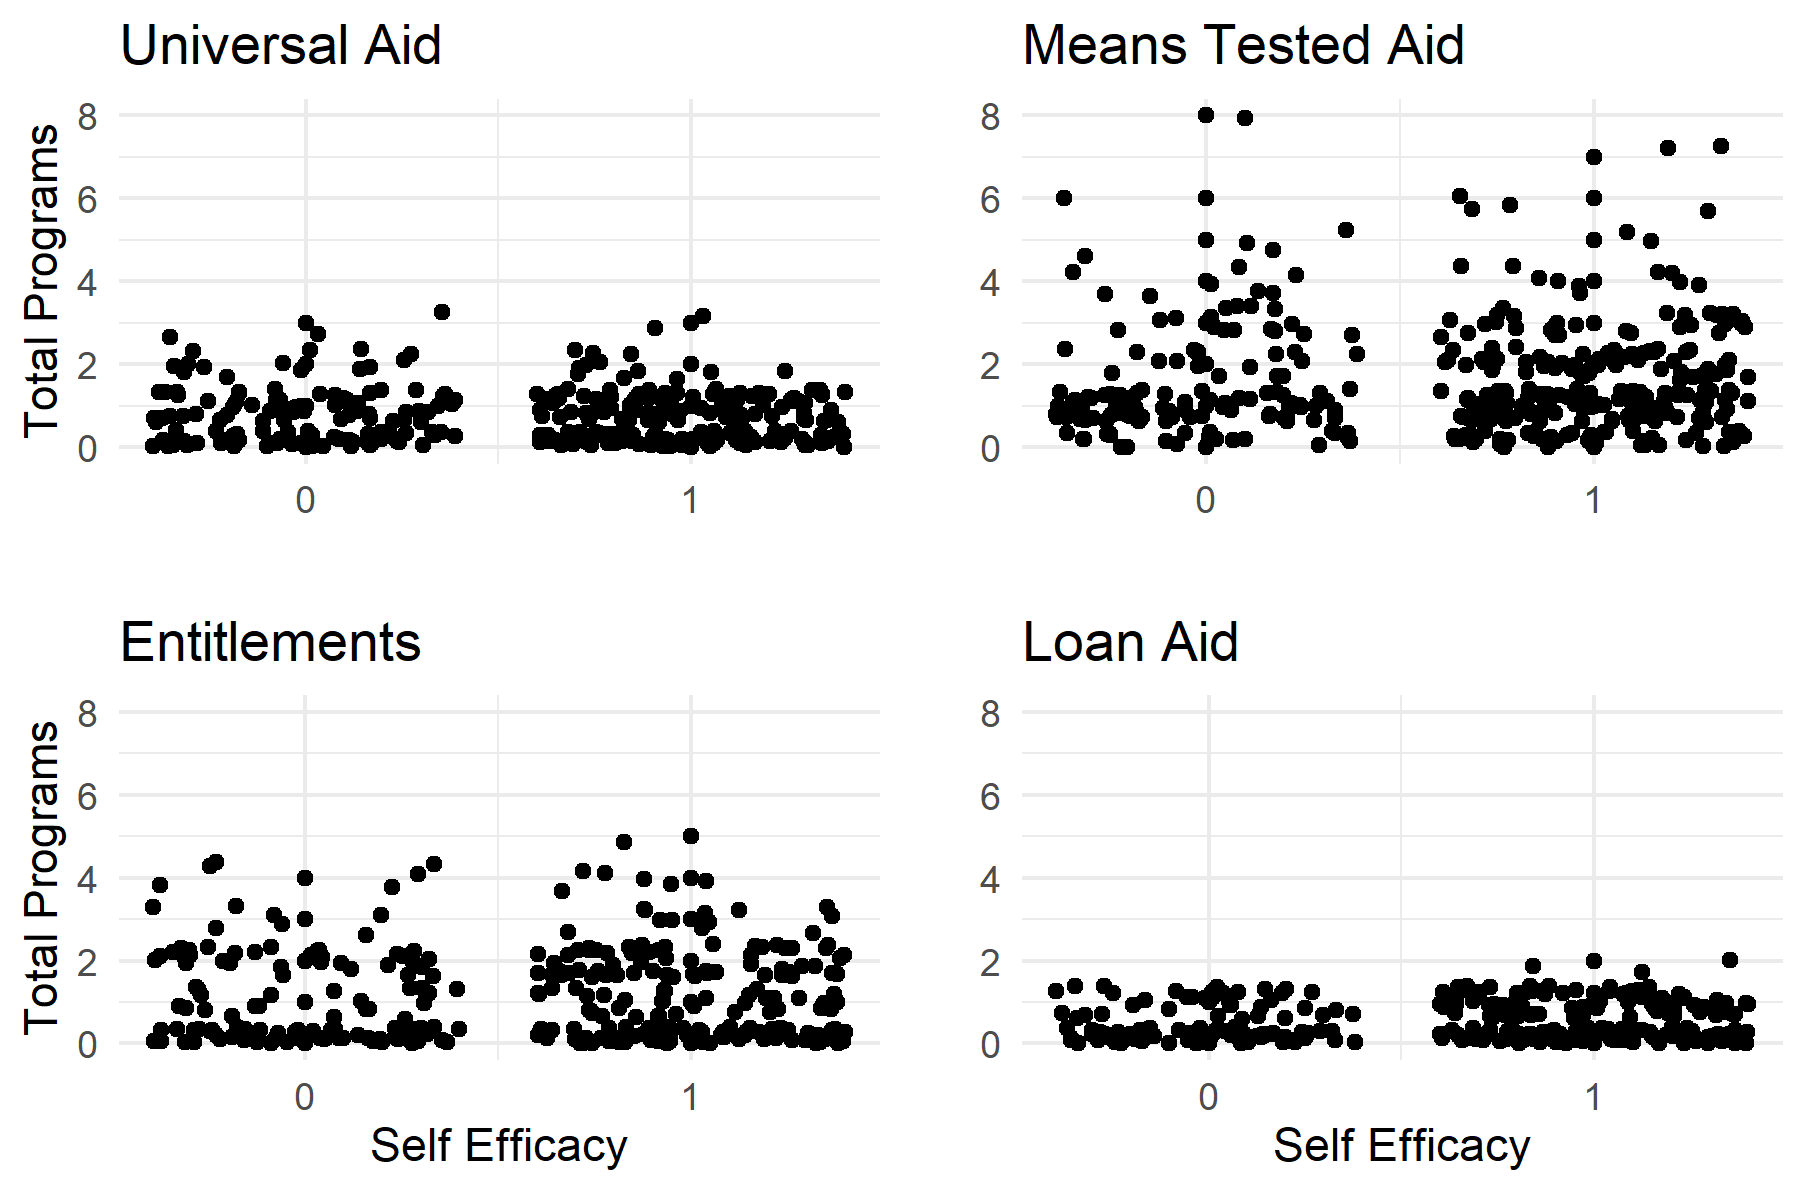
\includegraphics[width=.8\linewidth]{Figs/scatter_SE.png}
	\caption{Plot of Aid and Self Efficacy from the Maxwell Poll}
	\label{}
\end{figure}

With this more appropriate conceptualization of aid, I empirically evaluate the self efficacy mechanism. To do this, I look at the correlation between each aid type and self-reported self efficacy using the Maxwell Poll data from Mettler and Stonecash (2008).\footnote{The Maxwell Poll asks respondents, ``Do you agree or disagree with this statement: `People like me don’t have much say about what government does'?" Agree is coded as 0, indicating low self efficacy, while disagree is coded as 1, indicating high self efficacy.} As a first step, I plot the relationship between aid-type and self-efficacy. While there are more means-tested programs respondents could participate in, generally, respondents appear to report low and high self efficacy with similar frequencies across aid types. There is not an obvious association between aid type and self efficacy.

To further evaluate the self efficacy mechanism, I regress several measures of aid on self-reported self efficacy, testing the association between the aid a person receives and their self-reported self efficacy. The directional results and significance levels are reported in Table 2, but the full table with coefficients can be found in Appendix B. Both receiving aid and receiving \textit{more} aid are negatively associated with high self efficacy. This is consistent with the information perspective I proposed above, in which aid recipients have more information about government and have a lower evaluation of its responsiveness, and the self efficacy perspective, in which aid institutions diminish beneficiaries' self efficacy. However, in contrast to previous work, I find a negative and significant association between receiving universal aid and self efficacy $(p < 0.01)$. No other form of aid has a statistically significant effect on the likelihood of having low self efficacy, though the coefficient on the count of means-tested aid is appropriately signed. 

\begin{table}[!htbp] \centering 
	\begin{adjustbox}{width=1\textwidth}
		\begin{tabular}{@{\extracolsep{5pt}}lD{.}{.}{-3} D{.}{.}{-3} D{.}{.}{-3} D{.}{.}{-3} D{.}{.}{-3} D{.}{.}{-3} D{.}{.}{-3} } 
			\\[-1.8ex]\hline \\[-1.8ex] 
			\\[-1.8ex] & \multicolumn{7}{c}{Self Efficacy} \\ 
			\hline \\[-1.8ex] 
			Aid Dummy & -^{***} & -^{***} &  &  &  &  &  \\ 
			Total Aid &  &  & -^{**} &  &  &  &  \\ 
			Count: Total Universal Aid &  &  &  & -^{***} &  &  &  \\ 
			Count: Total Loans &  &  &  &  & + &  &  \\ 
			Count: Total Entitlements &  &  &  &  &  & - &  \\ 
			Count: Total Means-Tested &  &  &  &  &  &  & - \\ 
			Republican (dummy) & +^{***} & - & +^{***} & +^{***} & +^{***} & +^{***} & +^{***} \\ 
			Aid Dummy x Republican &  & + &  &  &  &  &  \\ 
			\hline \\[-1.8ex] 
			\multicolumn{8}{l}{$^{*}$p $<$ .1; $^{**}$p $<$ .05; $^{***}$p $<$ .01} \\
			\multicolumn{8}{l}{Standard errors are given in parentheses.} \\
			\multicolumn{8}{c}{All models include controls for sex, education, income, race, following public affairs, and trust in government. N=458.}   
		\end{tabular} 
	\end{adjustbox}
	\caption{The Relationship Between Aid and Self Efficacy} 
	\label{}
\end{table} 

In light these cursory results, the evidence for the self efficacy mechanism is murky.\footnote{I perform a cursory analysis of what drives this effect in Appendix B. While receiving all forms of universal aid included in my measure are associated with an decrease in self efficacy, this relationship is starkest among those receiving Social Security Disability Insurance (SSDI).} If receiving universal aid decreases the likelihood of having high self efficacy, how can low self efficacy be the mechanism by which aid depresses turnout only among voters receiving means-tested aid? Are our most common measures of self efficacy really capturing self efficacy or, as I suggest, are they capturing the effect of the specialized information to which aid beneficiaries are privy?

In the following section, I propose a theory of federal aid and voter behavior which does not depend on self efficacy as the mechanism by which aid depresses certain voters' turnout. My theory simply proposes that it is costly to voters to have an Executive who is distant from them on a spatial partisanship scale [0,1], but that tangible benefits from the Executive can offset these costs. I present the full mathematical model below but give a conceptual overview here. 

Following Gomez and Wilson (2003), voters credit the incumbent President with the distribution (or lack thereof) of aid prior to an election.\footnote{Gomez and Wilson (2003) demonstrate that, for most voters, the President is the figurehead of the government and is, therefore, the easiest attributive link between federal action and individual opinion. Therefore, while acknowledging that aid is a complex process involving federal, state, and bureaucratic actors, my model includes only the attributive relationship between the Voter (V) and the Incumbent (I).} Aid-receiving voters prefer Executives that prioritize aid-spending and especially prefer aid-prioritizing Executives that are in their political party $(|x_V - \theta_I| < \frac{1}{2})$. However, during elections, they cannot know whether the Incumbent is \textit{truly} an aid-prioritizing candidate. The best voters can do is make an educated guess based on the Incumbent's history of redistribution. If the Incumbent has delivered aid in the past, members of his party are motivated to turnout to reelect him. Members of the opposition party, however, are less motivated to turnout to vote against him.

This theory differs from existing models in several important ways. First, it treats turnout as the mechanism by which aid alters electoral outcomes. Previous work holds that aid alters electoral outcomes by altering vote choice (Cox and McCubbins 1986; Lindbeck and Weibull 1987; Stokes 2005).\footnote{In response to Stokes (2005), Nichter (2008) argues that Argentinian clientele parties are really buying turnout, not votes, but his empirical evidence is lacking. Further, the Stokes/Nichter debate concerns the ability of party operatives to observe or reasonably observe vote choice.} Dovetailing from this, the second novel component of this model is that it concerns all forms of public aid, meaning that goods are rarely targetable and that I allow the value of aid to vary continuously from [0,1]. The long-standing debate on how candidates should distribute targetable goods question pits Cox and McCubbins's (1986) ``core voter model” against Lindbeck and Weibull's (1987) ``swing voter model.” Cox and McCubbins argue that vote-maximizing parties will allocate distributive benefits primarily to their core voters - and not to their opposition. Meanwhile, the swing voter logic holds that ``voters who are predisposed in favor of [a party] on partisan or programmatic grounds [– that is, its core voters –] cannot credibly threaten to punish their favored party if it withholds [distributive] rewards. Therefore the party should not waste rewards on them," (Stokes 2005, 317). However, many federal aid programs are not targetable and, therefore, the effect of aid distribution may differ importantly from these classical predictions. In my theory, the Incumbent's distributive policy is exogenous from the voter's ideal point, meaning that aid is not targeted. I argue instead that alters electoral outcomes by altering voter turnout, not just vote choice. Empirically, this is convenient because, while vote choice is private, data on voter turnout is  accessible and allows my hypotheses to be more easily and rigorously tested. Further, in contrast to Nichter (2008), I demonstrate that candidates benefit by distributing aid even to their opposition.

In this vein, another unique advantage of my model is that my core argument - that partisanship will generally determine \textit{vote choice,} but factors like redistribution can affect \textit{voter turnout} - is supported by a rich body of literature on partisanship and swing voters. It is generally agreed upon that partisanship is an important factor when considering vote choice (Campbell et. al 1960; Achen and Bartels 2016), that "swing" voters are increasingly rare (Bitecofer 2018), and that inter-party polarization is on the rise (Abramowitz 2010; Iyengar et al. 2012; Ahler and Sood 2018). Thus, rather than argue that incumbents can buy their weak opposition with redistribution, I instead argue that they can mobilize their base and depress their opposition.

\section{A Formal Model of Aid and Attribution}
\textbf{Players:} Two politicians, an incumbent (I) and a challenger (C), who have different ideal points $(x_I=1, x_C=0)$.\footnote{By convention and for empirical convenience, I orient the model such that the Incumbent is a right-wing candidate (1) and the challenger is a left-wing candidate (0). We could invert the model for a left-wing Incumbent and right-wing Challenger.}  A voter (V) whose ideal point $x_V \epsilon [0,1]$ lies somewhere between $x_I$ and $x_C.$ When $x_V > \frac{1}{2}$, I consider her a right-wing voter. When $x_V < \frac{1}{2}$, I consider her a left-wing voter. Voters at $\frac{1}{2}$ abstain by assumption.

\textbf{Player Types:} Nature selects the politicians’ types, $\theta_I, \theta_C \epsilon \{0,1\}$, with probabilities: $Pr(\theta_I=0)=Pr(\theta_I=1)=Pr(\theta_C=0)=Pr(\theta_C=1)= \frac{1}{2}$ Nature privately reveals $\theta_I,\theta_C$ to I and C, respectively. Type $\theta=0$ prefers not to deliver aid, though delivers aid with some positive probability. Type $\theta=1$ prefers to deliver aid though fails to deliver aid with some positive probability. The probability that the politician delivers aid in accordance with his type is $p > 1 – p$ or $p > \frac{1}{2}$.\footnote{In the real world, politicians have some control over the types of aid they distribute. However, often, the need for aid, and the need for a certain kind of aid, is determined by apolitical circumstances, such as a hurricane, a stock market crash, or a pandemic. Because of this, I make the simplifying assumption that Incumbents' aid preferences are exogenous and that Incumbents do not always behave according to their type to mirror real-world pressures and constraints.}

\textbf{Sequence of Play}
\begin{enumerate}
	\item Nature determines each politician’s type, $\theta_I, \theta_C \epsilon \{0,1\},$ with probabilities $(\frac{1}{2}, \frac{1}{2})$ and reveals types privately to I and C, respectively.
	\item Incumbents pick the first period aid amount, $y_1\epsilon \{0,1\}.$ The incumbent behaves according to his type with probability \textit{p}. First period aid $y_1\epsilon \{0,1\}$ is administered.\footnote{Of course, not all aid is created equally. Some aid programs require impose a great administrative burden on potential beneficiaries in order to qualify. This burden - in the form of extensive employment and medical histories, visits and interviews with case workers, drug tests, etc. - may offset the value of the aid received. I consider this possibility in Appendix A, where I present a conceptual expansion of this model in which the aid delivered in $t_1$ varies continuously between $[0,1]$.}
	\item Nature determines the cost of voting, $c \epsilon U[0,1]$ and reveals this cost to voter V.
	\item The voter V chooses whether to vote, $v \epsilon \{0,1\}$
	\item If V votes $(v=1)$, then he decides the election winner, I or C. If V does not vote $(v=0)$, Nature decides the election winner, I or C.
	\item The winner (I or C) picks the second period aid amount, $y_2 \epsilon \{0,1\}$. The winner behaves according to his type with greater likelihood than not. Second period aid  $y_2 \epsilon \{0,1\}$ is administered.
\end{enumerate}

\textbf{Politicians' Utility}: In each period $t \epsilon \{1,2\}$, each politician $P \epsilon \{I,C\}$ receives:\footnote{This utility function relies on the assumption that politicians are interested strictly in what happens while they are in office. It does not incorporate a cost associated with losing (or payoff from winning) the election. In the future, we could expand this model to focus on the politicians' strategies and allow them to behave strategically. For the sake of focusing on voter behavior, however, I tie the hands of the politicians in this model and make their sole focus their distributive policy.} 

\begin{gather}
U_{p}^t = -|\theta_p - y_t|
\end{gather}

where $y_t\epsilon \{0,1\}$ is the executive’s choice of distributive aid policy. $\theta_p$ denotes the politician’s type, which represents her preferred distributive policy. Hence, a politician of type $\theta_p = 1$ prefers to deliver aid $(y_t = 1)$, while a politician of type $\theta_p = 0$ always prefers no aid $(y_t = 0).$

\emph{Voter's Utility}: V’s utility function is constant across periods: 
\begin{gather}
U_{V}^t = -|x_o - x_V| + y_t
\end{gather}

where $y_t \epsilon \{0,1\}$ represents the amount of distributive aid awarded to the voter in period $t \epsilon \{1,2\}$, $x_V$ represents the voter’s ideal point, and $x_o$ is the ideal point of the office-holding politician, who is either the Incumbent $(x_I = 1)$ or the Challenger $(x_C = 0).$ Hence, the voter’s utility depends on his partisan proximity to the office holder as well as his benefit from any distributive aid.

In between the two periods, the voter may choose to vote in the election by incurring a turnout cost, $c$, which is randomly drawn by Nature from the uniform distribution $c \epsilon U[0,1]$ and revealed to $V$ prior to the election. $V$’s payoff for the entire game is therefore given by:

\begin{gather}
U_{V}^1 + U_{V}^2 - c \times v
\end{gather}

where $v \epsilon \{0,1\}$ is V’s choice of whether to turn out in the election, and $U_{V}^1$ and $U_{V}^2$ are V’s payoffs from the first and second periods, respectively.

\emph{Voter Beliefs}: The Voter V does not observe the politician types, $\theta_I$ and $\theta_C$, that Nature randomly chooses. Instead, V can only observe the Incumbent's first-period distributive policy,  $y_1$, and form updated beliefs about I’s type. Let $p_{\theta_I} (\theta_p | y_1 )$ denote the V’s posterior beliefs about the probability that $\theta_I = 1$ after observing $y_1$.

\subsection{Equilibria}
For simplicity, I assume that Voter V resolves indifference in favor of abstaining. For proofs, see Appendix D.
	
\textbf{Lemma 1:} In each period $t \epsilon \{1,2\}$, the office-holding executive, $p \epsilon \{I,C\}$, chooses the distributive policy: 
\begin{gather}
x_t=\theta_j (1-p)+ \theta_i (p), 
\end{gather}

where $\theta_j$ is the opposite of the office holder’s type. Incumbent types are therefore not fully separating.

\textbf{Lemma 2:}  After observing the Incumbent’s choice of $y_1 \epsilon {0,1}$ during the first period, the Voter V’s updated belief about the Incumbent’s type is: 
\begin{gather}
p_{(\theta_I)}(p(\theta_i ) + (1 - p)(\theta_j ) | y_1 )=y_1(p)
\end{gather}

V’s expected second period payoff from I’s reelection would be: $EU_V (e=I) = -(1 - x_v ) + [p(y_1 ) + (1 - p)(y_1 )]$ whereas his expected second period payoff from C’s election would be: $EU_V (e=C) = - x_V + \frac{1}{2}$. 

Conditional on turning out, V votes for I iff: 
\begin{gather}
x_V \geq -\frac{3 - 2py_1 - 2y_{-1} - 2py_{-1}}{4}
\end{gather}

When $x_V$ is above the threshold, V prefers that the Incumbent win the election, so V’s total expected payoff from voting would be:
\begin{gather}
 EU_V (v=1 | x_V \geq -\frac{3 - 2py_1 - 2y_{-1} - 2py_{-1}}{4} =
  - (1 - x_V ) + y_1 - c
\end{gather}

When $x_V$ is below the threshold, V prefers that the Challenger win the election, so V’s total expected payoff from voting would be:
\begin{gather}
 EU_V (v=1 | x_V < -\frac{3 - 2py_1 - 2y_{-1} - 2py_{-1}}{4} = 
  -x_V + \frac{1}{2} - c
\end{gather}

V’s total combined expected payoff from not voting is:
\begin{gather}
EU_V (v=0) = 
\frac{y_1}{2} - \frac{1}{4}
\end{gather}

Hence, V turns out to vote iff: $EU_V (v=1) \geq EU_V (v=0) \Rightarrow c \leq \bar{c}$ where:

\begin{equation}
\bar{c} =
\begin{cases}
\frac{-y_1}{2} - x_V + \frac{3}{4} & if x_V < \frac{1}{4} \\
x_V (2y_1 - 1) + \frac{3}{4}     & if \frac{1}{4} \leq x_V < \frac{3}{4}  \\
\frac{y_1}{2} + x_V - \frac{3}{4}     & if x_V \geq \frac{3}{4}  \\
\end{cases}
\end{equation}

\textbf{Lemma 3:}
Given turning out, V’s vote in the election is:
\begin{equation}
s =
\begin{cases}
I, & if x_V \geq -\frac{3 - 2py_1 - 2y_{-1} - 2py_{-1}}{4} \\    
C,     & otherwise  \\
\end{cases}
\end{equation}
where $y_{-1}$ is the aid amount not delivered in the period (i.e. if $1$ unit of aid was delivered, $y_{-1} = 0$.) 

This demonstrates the consequence of candidate types not fully separating in equilibrium: it is entirely possible that the Voter could oust an Incumbent of type $\theta_I = 1$ and keep an incumbent of type $\theta_I = 0$ due to a bad signal.\footnote{If the Incumbent's actions were not determined probabalistically, but were instead allowed to vary their aid policy strategically, it follows, then, that Incumbents would deliver the minimum amount of aid necessary to satisfy the Voter's threshold for $x_v > \frac{1}{2}$ and the minimum amount of aid necessary to repress turnout for $x_v < \frac{1}{2}$.}


\textbf{Lemma 4:} Let $Q(y_1 )(x_V )$ denote the probability of turnout for a voter with ideal point $x_V$ and who receives $y_1 \epsilon \{0,1\}$ of aid during Period 1. V’s turnout choice in the election is:

\begin{equation}
Q(y_1 )(x_V ) =
\begin{cases}
\frac{-y_1}{2} - x_V + \frac{3}{4} & if x_V < \frac{1}{4}\\    
x_V (2y_1 - 1) + \frac{3}{4}     & if \frac{1}{4} \leq x_V < \frac{3}{4}  \\
\frac{y_1}{2} + x_V - \frac{3}{4}     & if x_V \geq \frac{3}{4}  \\
\end{cases}
\end{equation}

Given this, we can calculate the \emph{change in turnout probability} from receiving one unit of aid in $t_1$. Put differently, the effect of receiving $y_1 = 1$ is:
\begin{equation}
Q_1 (x_V ) - Q_0 (x_V )=
\begin{cases}
\frac{-1}{2} & if x_V < \frac{1}{4}\\    
2x_V - 1 & if \frac{1}{4} \leq x_V < \frac{3}{4}  \\
\frac{1}{2} & if x_V \geq \frac{3}{4}  \\
\end{cases}
\end{equation}

In other words, delivering aid to distant voters on the partisan scale $(x_V < \frac{1}{2})$ strictly decreases their probability of turning out, while delivering aid to proximate voters on the partisan scale $(x_V > \frac{1}{2})$  strictly increases their probability of turning out. Additionally, conditional upon turnout, delivering aid strictly increases the likelihood of voting for the incumbent. The delivery of aid during period one increases V’s expected payoff from having the incumbent reelected relative to the probability that the aid distribution was an informative signal. The increased expected payoff drives my main prediction that the delivery of aid in period one increases a right-wing voter's probability of turnout.

From Lemmas 1, 2, 3, and 4 we know that those who favor the Incumbent \emph{a priori} credit the Incumbent with the positive experience of aid and, therefore, turnout to vote for him or her. Those who do not favor the incumbent \emph{a priori}, rather than change their vote choice, are simply less motivated to turnout to oust the Incumbent. Distant voters, therefore, should be less likely to turnout to vote at all. Put differently, receiving aid in $t_1$ causes a relatively larger increase in a right-wing voter’s turnout probability but a relatively smaller decrease in a left-wing voter’s turnout probability, given $p > \frac{1}{2}$. If my model paints a useful picture of the world, we should expect to observe the following:

\emph{$H_1:$ For a left-wing voter $(x_V < \frac{1}{2})$, receiving distributive aid in period 1 causes a strict decrease in the probability of voter turnout.}

\emph{$H_2$: For a right-wing voter $(x_V > \frac{1}{2})$, receiving distributive aid in period 1 causes a strict increase in the probability of voter turnout.}

\subsection{Expansion}
Of course, not all aid is created equally.Incumbents may deliver aid to constituents in a way that forces potential recipients to incur a cost, such as means-testing, gathering records to confirm eligibility, or other administrative burdens on potential beneficiaries. Contrastingly, consider COVID-19 individual aid, for which individuals did not have to apply.

To account for heterogeneity in administrative costs, we might allow the value of aid to vary continuously between 0-1. When the Incumbent delivers one unit of aid, regardless of his type, we can write this aid amount as $1 – \delta$, where $\delta \epsilon [0,1]$ and represents the personal, psychological, social, and administrative costs of obtaining aid. There may be no cost to participants to obtain aid $(\delta = 0)$; alternatively, the cost of obtaining aid may negate any potential benefit $(\delta = 1)$. Thus, the voter’s expected utility is given by $U_{V}^t = -|x_o - x_V| + [y_t - \delta]$. When $(\delta = 0)$, the expanded model is identical to the original. When $(\delta > 0)$, however, $\delta$ impedes the ability of aid to offset the cost of voting for the incumbent. For simplicity, I represent $y_t - \delta$ as  $\lambda_t$. Now, not only is incumbent type determined exogenously, but so is the value of aid.


The politicians’ utility is still given by,

\begin{gather}
U_{p}^t = -|\theta_p - y_t|
\end{gather}

because the Incumbent does not incur the cost associated with aid. That cost is transferred onto the voter.

The voter’s utility in each period is now given by, 
\begin{gather}
U_{V}^t = -|x_o - x_V| + \lambda_t
\end{gather}

Previously, $y_t \epsilon \{0,1\}$ had either no effect $(y_t = 0)$ or a strictly positive effect $(y_t = 1)$ on V's utility. Now, both $x_V$ and $\lambda_t$ vary continuously between 0 and 1. If $\lambda_t < |x_o - x_V|$, aid will not have a positive effect on V’s utility per round. 

Given that aid is delivered, I assume voters expect $\lambda_t$ to remain constant across candidates. That is, while the deliverance of aid or no aid may vary between rounds, administrative costs should remain constant if the Incumbent remains in power. If voters receive aid in $t_1$ at some value $\lambda_t$, they update their beliefs about the Incumbent based on the expected probability of receiving 0 or $\lambda_t$.

I present the formalized model in Appendix A. For brevity, I discuss only its intuition here. As $\delta$ increases (or as $\lambda$ decreases), so does aid's effect on turnout and vote choice. Recall in the baseline model that aid has a strictly negative effect on turnout for left-wing voters $(x_V < \frac{1}{2})$ and a strictly positive affect on right-wing voters $(x_V > \frac{1}{2})$. When aid is allowed to vary continuously, this is no longer the case. Now, only aid that is at or above some threshold will influence vote and turnout choice. For the left-wing voter, turnout probability is \textit{increasing} as $\delta$ increases. For the right-wing voter, turnout probability is \textit{decreasing} as $\delta$ increases.

\textit{$H_3$: For the left-wing voter $(x_V < \frac{1}{2})$, those participating in aid with low administrative costs will be less likely to turnout to vote than those participating in aid with high administrative costs.}

\textit{$H_4$: For a right-wing voter $(x_V > \frac{1}{2})$, those participating in aid with low administrative costs will be more likely to turnout to vote than those participating in aid with high administrative costs.}

\section{Research Design}
To test the implications of my model, I use data from the Maxwell Poll on Citizenship and Inequality from Syracuse University, directed by Jeffery Stonecash. The poll includes data on federal aid status, voter behavior, and civic engagement. The poll is nation-wide annual survey and was administered by phone from 2004-2007. The cumulative data file from the surveys contain weights so that the data is nationally representative and each year averages approximately 600 respondents. I conduct my analysis using binary and ordered logit models, but my results are robust to OLS estimation (see Appendix B). My dependent variable is turnout. The Maxwell Poll asks respondents whether they turnout Always (4), Often (3), Sometimes (2), or Not at all (1). I use this ordinal measure of turnout as well as a binary measure in which I code those who respond ``Always" and ``Often" as 1 and those who responded ``Sometimes" and ``Never" as 0.

My primary independent variable is receiving government aid. I employ three measures of aid across different models to account for heterogeneity within aid programs and account for the cumulative effect of aid on voter behavior. First, I create a binary variable in which 1 means the respondent or a member of the respondent’s household receives any form of government assistance and a 0 means no one in the household receives government assistance. Second, I use my novel measure of aid-types that I introduced in Section 2: the counts of the total number of entitlement, means-tested, universal, and subsidized loan aid the household receives. A 0 in all four categories would mean the respondent’s household receives no aid. This allows me to test $H_3$ and $H_4$, since in general loans and means tested aid have a more strenuous application process, while entitlements and universal aid programs are, on average, easier to enroll in. Finally, I measure aid continuously as the count of total aid programs in which a person participates. Descriptive statistics for my key variables can be found in Appendix B.

For Party ID, I use a binary measure in which a 1 is Republican and a 0 is Democrat. I also include a battery of controls in each model, including race, income, education, sex, how closely the person follows public events, their trust in public officials, and their sense of their self efficacy.

\section{Analysis}

Recall $H_1$ and $H_2$ assert that receiving aid \textit{and} party ID cause a change in turnout. Since the incumbent president during the time of the survey is George W. Bush (R), I predict that Republicans who receive aid will be more likely to turnout than Democratic voters who receive aid. To test my hypotheses, I first use the dummy variable for aid, which takes on a value of 1 if the respondent benefits from any of the federal aid programs asked about in the survey and 0 otherwise. Using this as my primary independent variable, I estimate a model that interacts Party ID and the Aid Dummy. The results of both the binary and ordered logit for both models are shown in Table 3.

%%Model 3: Vote ~ recieves aid dummy**partyID + controls
\begin{table}[!htbp] \centering 
\begin{adjustbox}{width=1\textwidth}
\begin{tabular}{@{\extracolsep{5pt}}lD{.}{.}{-3} D{.}{.}{-3} }
\\[-1.8ex]\hline \\[-1.8ex] 
\\[-1.8ex] & \multicolumn{1}{c}{Vote Dummy} & \multicolumn{1}{c}{Vote Frequency (1-4)} \\ 
\\[-1.8ex] & \multicolumn{1}{c}{(1)} & \multicolumn{1}{c}{(2)}\\ 
\hline \\[-1.8ex] 
Aid Dummy & 2.755^{***} & 1.058^{*} \\ 
& (0.819) & (0.619) \\ 
Republican & 16.727 & 1.323 \\ 
& (819.837) & (0.955) \\ 
Aid Dummy x Republican & -16.630 & -1.362 \\ 
& (819.837) & (0.983) \\ 
Constant & -0.518 &  \\ 
& (1.161) &  \\ 
N & \multicolumn{1}{c}{458} & \multicolumn{1}{c}{480} \\ 
Log Likelihood & \multicolumn{1}{c}{-128.697} &  \\ 
AIC & \multicolumn{1}{c}{277.395} &  \\ 
\hline \\[-1.8ex] 
\multicolumn{3}{l}{$^{*}$p $<$ .1; $^{**}$p $<$ .05; $^{***}$p $<$ .01} \\
\multicolumn{3}{l}{Standard errors are given in parentheses.} \\
\multicolumn{3}{c}{All models include controls for sex, education, income, race, self efficacy, following public affairs, and trust in government.}   

\end{tabular}
\end{adjustbox}
\caption{Aid and Party ID} 
\label{}
\end{table} 

The aid dummy and Republican are positively signed, as predicted in $H1$ and $H2$. However, the interaction between the two is neither significant nor signed as expected. The marginal effects of aid for Democrats are positive while they are negative for Republicans. Thus, I fail to find support for $H_1$ and $H_2$ in Model 2. In fact, I find the opposite. Aid-receiving Democrats are more likely to turnout to vote frequently, all else held constant at 0.

I also measure aid continuously as the count of total aid programs in which a person participates. I interact this total aid measure on party ID in Table 4. As before, the measures of aid and Republican are signed as predicted, but the coefficient on the interaction term is negative. The marginal effect of aid is once again the opposite of what $H_1$ and $H_2$ predict. Again, I do not find support for my hypotheses.

If my model usefully reflects the world we live in, those who favor the incumbent \textit{a priori} should be more likely to credit the incumbent with the positive experience of aid and, therefore, turnout to vote for him or her. Those who do not favor the incumbent \textit{a priori} may credit the incumbent with the positive experience of aid, but be unwilling to vote for a candidate from a party they do not prefer. Voters engaging in this attributive process, therefore, should be less likely to turnout to vote at all. Across empirical tests, however, these predictions do not hold. In 2004-2007, receiving aid and being Republican are generally associated with higher turnout, but aid-receiving Republicans have a lower estimated likelihood of turnout than Republicans receiving no aid or aid-receiving Democrats.

%%Model 9-10 - Total Aid and Total Aid*PID interaction
\begin{table}[!htbp] \centering 
	\begin{adjustbox}{width=1\textwidth}
		\begin{tabular}{@{\extracolsep{5pt}}lD{.}{.}{-3} D{.}{.}{-3} D{.}{.}{-3} D{.}{.}{-3} } 
			\\[-1.8ex]\hline \\[-1.8ex] 
			\\[-1.8ex] & \multicolumn{1}{c}{Vote Frequency (1-4)} & \multicolumn{1}{c}{Vote Dummy} & \multicolumn{1}{c}{Vote Frequency (1-4)} & \multicolumn{1}{c}{Vote Dummy} \\  
			\\[-1.8ex] & \multicolumn{1}{c}{(1)} & \multicolumn{1}{c}{(2)} & \multicolumn{1}{c}{(3)} & \multicolumn{1}{c}{(4)}\\ 
			\hline \\[-1.8ex] 
			Total Aid & -0.002 & 0.159^{*} & 0.030 & 0.249^{**} \\ 
			& (0.047) & (0.089) & (0.064) & (0.118) \\ 
			Republican (dummy) & 0.028 & 0.338 & 0.264 & 1.061 \\ 
			& (0.211) & (0.387) & (0.392) & (0.697) \\ 
			Total Aid x Republican &  &  & -0.065 & -0.232 \\ 
			&  &  & (0.090) & (0.180) \\ 
			Constant &  & 0.859 &  & 0.763 \\ 
			&  & (1.002) &  & (1.012) \\ 
			N & \multicolumn{1}{c}{480} & \multicolumn{1}{c}{458} & \multicolumn{1}{c}{480} & \multicolumn{1}{c}{458} \\ 
			Log Likelihood &  & \multicolumn{1}{c}{-133.086} &  & \multicolumn{1}{c}{-132.182} \\ 
			AIC &  & \multicolumn{1}{c}{284.171} &  & \multicolumn{1}{c}{284.363} \\ 
			\hline \\[-1.8ex] 
			\multicolumn{5}{l}{$^{*}$p $<$ .1; $^{**}$p $<$ .05; $^{***}$p $<$ .01} \\
			\multicolumn{5}{l}{Standard errors are given in parentheses.} \\
			\multicolumn{5}{c}{All models include controls for sex, education, income, race, self efficacy, following public affairs, and trust in government.}   
		\end{tabular} 
	\end{adjustbox}
	\caption{Total Aid} 
	\label{}
\end{table} 

This may be due to differences in the costs different aid programs impose on their participants. Some aid programs require detailed income and wealth information, medical and employment histories, monthly interviews, and quarterly reevaluation of eligibility. The costs these programs impose on beneficiaries may diminish the effect of aid on turnout ($H_3$ and $H_4$). In general, government loan programs and means-tested programs impose the highest costs on participants. Entitlements and universal aid programs tend to be easier, on average, for potential beneficiaries to apply for.

In Table 5, I use counts of each of the four types of aid programs as my dependent variables. I predicted that high-cost aid programs, like loans and means-tested aid, would decrease turnout among Republicans and increase aid among Democrats, and that low-cost aid programs, like universal aid and entitlements, would increase turnout among Republicans and decrease aid among Democrats. I find the opposite to be true. Receiving more entitlements are associated with an increase in turnout likelihood in Democrats and associated with a decrease in turnout likelihood among Republicans.

\begin{table}[!htbp] \centering 
	\begin{adjustbox}{width=1\textwidth}
\begin{tabular}{@{\extracolsep{5pt}}lD{.}{.}{-3} D{.}{.}{-3} D{.}{.}{-3} D{.}{.}{-3} D{.}{.}{-3} } 
	\\[-1.8ex]\hline \\[-1.8ex] 
	\\[-1.8ex] & \multicolumn{5}{c}{Vote Dummy} \\ 
	\\[-1.8ex] & \multicolumn{1}{c}{(1)} & \multicolumn{1}{c}{(2)} & \multicolumn{1}{c}{(3)} & \multicolumn{1}{c}{(4)} & \multicolumn{1}{c}{(5)}\\ 
	\hline \\[-1.8ex] 
	Total Loans & 0.766^{*} & 0.387 &  &  &  \\ 
	& (0.444) & (0.478) &  &  &  \\ 
	Total Universal Aid & 0.492 &  &  & 0.456 &  \\ 
	& (0.342) &  &  & (0.379) &  \\ 
	Total Entitlements & 0.326 &  & 1.702^{**} &  &  \\ 
	& (0.234) &  & (0.739) &  &  \\ 
	Total Means-Tested Aid & -0.089 &  &  &  & 0.048 \\ 
	& (0.145) &  &  &  & (0.148) \\ 
	Republican & 0.288 & 0.125 & 0.902^{**} & 0.238 & 0.310 \\ 
	& (0.393) & (0.427) & (0.453) & (0.446) & (0.514) \\ 
	Total Loans x Republican &  & 0.978 &  &  &  \\ 
	&  & (0.927) &  &  &  \\ 
	Total Entitlements x Republican &  &  & -1.939^{**} &  &  \\ 
	&  &  & (0.788) &  &  \\ 
	Total Universal Aid x Republican &  &  &  & 0.244 &  \\ 
	&  &  &  & (0.676) &  \\ 
	Total Means-Tested Aid x Republican &  &  &  &  & 0.036 \\ 
	&  &  &  &  & (0.289) \\ 
	Constant & 0.790 & 1.332 & 1.173 & 1.339 & 1.346 \\ 
	& (1.049) & (0.968) & (1.009) & (0.962) & (0.981) \\ 
	N & \multicolumn{1}{c}{458} & \multicolumn{1}{c}{458} & \multicolumn{1}{c}{458} & \multicolumn{1}{c}{458} & \multicolumn{1}{c}{458} \\ 
	Log Likelihood & \multicolumn{1}{c}{-130.858} & \multicolumn{1}{c}{-132.550} & \multicolumn{1}{c}{-125.237} & \multicolumn{1}{c}{-132.572} & \multicolumn{1}{c}{-134.406} \\ 
	AIC & \multicolumn{1}{c}{285.715} & \multicolumn{1}{c}{285.100} & \multicolumn{1}{c}{270.474} & \multicolumn{1}{c}{285.145} & \multicolumn{1}{c}{288.811} \\ 
	\hline \\[-1.8ex] 
	\multicolumn{6}{l}{$^{*}$p $<$ .1; $^{**}$p $<$ .05; $^{***}$p $<$ .01} \\
	\multicolumn{6}{l}{Standard errors are given in parentheses.} \\
	\multicolumn{6}{c}{All models include controls for sex, education, income, race, self efficacy, following public affairs, and trust in government.}   
		\end{tabular} 
\end{adjustbox}
\caption{Count of Types of Aid} 
\label{}
\end{table} 

\section{Discussion}
Why do aid-receiving voters turn out at such low rates? After examining the evidence, the answer is less clear than previous work suggests. I empirically evaluate the mechanism by which some aid is theorized to depress turnout and find no support for it. However, I also fail to find support for my hypotheses that partisanship determines whether aid depresses or increases turnout likelihood. Despite failing to find support for my hypotheses, this paper makes several valuable contributions to the literature. First, it offers the first empirical test of the self efficacy hypothesis. Secondly, I present a novel categorization method for future scholars studying aid. My method groups aid intuitively, while providing for nuance than the traditional dichotomy. Finally, using my novel measure, I test the effect of aid-type on voter turnout. Counterintuitively, I find that Republicans receiving entitlements are less likely to turnout than Republicans who receive less entitlements, on average.

My work also has three important implications for future work on redistribution and voter behavior in the American context. First, future work would benefit from more suitable data to reevaluate my hypotheses. There is a great need for detailed, individual-level data on aid that is presently only available via a lengthy Freedom of Information Act (FOIA) request process. While the Maxwell Poll has been a valuable resource to scholars, self-reported turnout frequency is a poor approximation of voter turnout. Better data are needed to fully understand the relationship between aid and turnout.

Secondly, future work should consider new ways to reevaluate and measure the self efficacy hypothesis, as my work suggests that it is less straightforward of a mechanism than political scientists believed. While my cursory analysis is certainly not a fatal bullet in the self efficacy hypothesis, it highlights that the mechanism does not behave as excepted and is not robust to more valid constructs of aid.

Thirdly and finally, future work would benefit from further expansions of this theoretical model. Due to the focus of this paper, my discussion of my model ties the hands of the political actors and focuses almost exclusively on voters. Future work should consider the strategic actions of candidates who wish to maximize their vote share. Subsequent work would also benefit from considering how heterogeneous views on aid might influence politician's messaging about aid and voters' response to it.
%\bibliographystyle{APSR}
%\bibliography{references.bib}

\clearpage

\section*{Works Cited}
\singlespace 
\begin{hangparas}{.25in}{1}

Abramowitz, Alan I. 2010. ``Transformation and polarization: The 2008 presidential election and the new American electorate." \textit{Electoral Studies} 29(4): 594-603.

Ahler, Douglas J., and Gaurav Sood. 2018. ``The parties in our heads: Misperceptions about party composition and their consequences." \textit{The Journal of Politics} 80(3): 964-981.

Arceneaux, Kevin. 2006. ``The Federal Face of Voting: Are Elected Officials Held Accountable for the Functions Relevant to Their Office?’’ \textit{Political Psychology} 27 (5): 731–54.

Bitecofer, Rachel. 2018. ``What (Really) Happened." In \textit{The Unprecedented 2016 Presidential Election,} pp. 141-186. Palgrave Macmillan, Cham.

Campbell, Angus, Philip E. Converse, Warren E. Miller, and Donald E. Stokes. 1980. \textit{The American Voter.} University of Chicago Press.

Chen, Jowei. 2013. ``Voter partisanship and the effect of distributive spending on political participation." American Journal of Political Science 57(1): 200-217.

Conover, Pamela Johnston, Stanley Feldman, and Kathleen Knight. 1986. ``Judging Inflation and Unemployment: The Origins of Retrospective Evaluations." \textit{The Journal of Politics} 48(3): 565-88

Cox, Gary W., and Mathew D. McCubbins. 1986. ``Electoral politics as a redistributive game." \textit{The Journal of Politics} 48(2): 370-389.

Dowding, Keith. 2005. ``Is it rational to vote? Five types of answer and a suggestion.” \textit{British Journal of Politics and International Relations.} 7:442–459.

Feddersen, Timothy and Alvaro Sandroni. 2006. ``A theory of participation in elections." \textit{American Economic Review}, 96 (4): 1271-82

Gomez, Brad T. and J. Matthew Wilson. 2001. ``Political sophistication and economic voting in the American electorate: A theory of heterogeneous attribution.” \textit{American Journal of Political Science} 45:899-914.

Gomez, Brad T., and J. Matthew Wilson. 2003. ``Causal attribution and economic voting in American congressional elections." \textit{Political Research Quarterly} 56(3):271-282.

Hansford, Thomas and Brad Gomez. 2015. ``Reevaluating the Sociotropic Economic Voting Hypothesis.” \textit{Electoral Studies}. 39(10).

Iyengar, Shanto, Gaurav Sood, and Yphtach Lelkes. 2012. ``Affect, not ideology: A social identity perspective on polarization." \textit{Public Opinion Quarterly} 76(3): 405-431.

Johnson, James. 2020. ``Models-as-fables: An alternative to the standard rationale for using formal models in political science." \textit{Perspectives on Politics}: 1-16.

Labonne, Julien. 2013. ``The Local Electoral Impacts of Conditional Cash Transfers: Evidence from a Field Experiment.” \textit{Journal of Development Economics} 104 (September): 73–88.

Lindbeck, Assar, and Jörgen W. Weibull. 1987. ``Balanced-budget redistribution as the outcome of political competition." \textit{Public choice} 52(3): 273-297.

Lipset, Seymour Martin. 1960. \textit{Political Man: The Social Bases of Politics.} New York. 

Madsen, Douglas. 1987. ``Political self efficacy Tested.” \textit{American Political Science Review.} 81(2):571–81.

Manacorda, Marco, Edward Miguel, and Andrea Vigorito. 2011. ``Government Transfers and Political Support.” \textit{American Economic Journal: Applied Economics} 3(3): 1–28.

Mettler, Suzanne, and Jeffrey Stonecash. 2008. ``Government Program Usage and Political Voice.” \textit{Social Science Quarterly}. 89: 273-293. 


Pateman, Carole. 1970. \textit{Participation and Democratic Theory. }Cambridge, MA: Cambridge University Press.


Piven, Frances Fox, and Richard A. Cloward. 1971. \textit{Regulating the Poor.} New York: Vintage Books.


Pop-Eleches, Cristian, and Grigore Pop-Eleches. 2012. ``Targeted Government Spending and Political Preferences.” \textit{Quarterly Journal of Political Science} 7 (3): 285–320.


O, Ana L. De La. 2013. ``Do Conditional Cash Transfers Affect Electoral Behavior? Evidence from a Randomized Experiment in Mexico.” \textit{American Journal of Political Science} 57 (1): 1–14.


Olson, Mancur. 1965. \textit{The Logic of Collective Action.} Cambridge, MA: Harvard University Press

Rubinstein, Ariel. 1991. ``Comments on the interpretation of game theory." \textit{Econometrica: Journal of the Econometric Society}: 909-924.

Rubinstein, Ariel. 2006. ``Dilemmas of an economic theorist." \textit{Revista de Economía Institucional} 8(14): 191-213.

Soss, Joe. 1999. ``Lessons of Welfare: Policy Design, Political Learning, and Political Action.” \textit{The American Political Science Review} 93(2): 363-380.

Stokes, Susan C. 2005. ``Perverse Accountability: A Formal Model of Machine Politics with Evidence from Argentina.” \textit{American Political Science Review } 99(3): 315–25.


Verba, Sidney, Kay Lehman Schlozman, and Henry E. Brady. 1995. \textit{Voice and Equality: Civic Voluntarism in American Politics.} Cambridge, MA: Harvard University Press.

U.S. Census Bureau. 2012. ``Voting and Registration in the Election of November 2012 - Detailed Tables.” Census.gov. Retrieved: 11/10/2020.
\end{hangparas}
\clearpage


\section*{Appendix A - Expanded Model}
\textbf{Voter Beliefs}: The Voter V does not observe the politician types, $\theta_I$ and $\theta_C$, that Nature randomly chooses. Instead, V can only observe the Incumbent's first-period distributive policy,  $\lambda_1$, and form updated beliefs about I’s type.  For the Voter to update, I assume voters treat $\lambda_1 > 0$ as evidence that $\theta_I = 1$. Thus, $p_{\theta_I} (\theta_p | \lambda_1 )$ denote the V’s posterior beliefs about the probability that $\theta_I = 1$ after observing $\lambda_1$. This is because observing any nonzero unit of aid suggests an Incumbent of Type 1, but recall that $\lambda = 1 - \delta$. If $\delta$ is sufficiently high, the Voter will not receive the signal that the Incumbent has delivered aid.

Incumbent types remain probabalistically separating in equilibrium.

V expects to receive $E(\lambda_2 | e=I) = p(\lambda_i) + (1-p)(\lambda_j)$ units of aid in $t_2$ if the Incumbent is reelected. This is because I assume that administrative barriers are constant under the Incumbent. That is, if V received $\lambda_1 > 0$ in $t_1$, he anticipates receiving either $0$ or $\lambda_1$ in $t_2$, but not some other value of $\lambda$ because $\delta_I$ is fixed for the Incumbent.

If, however, C wins the election, Nature draws a new cost of aid, $\delta_C \epsilon [0,1]$. Thus, V expects to receive $E(\lambda_2 | e=C) = E(\theta_C) = \frac{1}{2}$ units of aid if C wins the election.

V’s expected second period payoff from I’s reelection is: 
\begin{gather}
EU_v(e = I) = -(1 - x_V) + [p(\lambda_i) + (1-p)\lambda_j] 
\end{gather}

Whereas his expected payoff from C's reelection is:
\begin{gather}
EU_v(e = C) = -x_V + \frac{1}{2}
\end{gather}

Conditional on turning out, $x_V$ votes for I iff:

\begin{gather}
EU_v(e = I) \geq EU_v(e = C) \rightarrow 
-(1 - x_V) + [p(\lambda_i) + (1-p)\lambda_j] \geq -x_V + \frac{1}{2} \rightarrow 
\lambda_i \geq \frac{3 - 4x_V - 2\lambda_j + 2p\lambda_j}{2p}
\end{gather}

When $x_V$ is above the threshold, the Voter prefers the Incumbent win the election. V's total expected payoff from voting is:
\begin{gather}
EU_v(v = 1 | \lambda_i \geq \frac{3 - 4x_V - 2\lambda_j + 2p\lambda_j}{2p}) =
-(1 - x_V) + \lambda_1 - c
\end{gather}

When $x_V$ is below the threshold, the Voter prefers the Challenger win the election. V's total expected payoff from voting is:
\begin{gather}
EU_v(v = 1 | \lambda_i < \frac{3 - 4x_V - 2\lambda_j + 2p\lambda_j}{2p}) = 
-x_V + \frac{1}{2} - c
\end{gather}

The total expected payoff of not voting is,
\begin{gather}
EU_V (v=0) = \frac{EU_V (e=I)}{2} + \frac{EU_V (e=C)}{2} =
 \frac{- (1 - x_V ) + \lambda_1}{2} + \frac{-x_V + \frac{1}{2}}{2} = 
 \frac{\lambda_1}{2} - \frac{1}{4}
\end{gather}

\clearpage

\section*{Appendix B - Tables}
\subsection*{Full Tables}
In this section, I present the full tables from the body of the paper. These tables include all coefficients and control variables.

\begin{table}[!htbp] \centering 
	\begin{adjustbox}{width=1\textwidth}
		\begin{tabular}{@{\extracolsep{5pt}}lD{.}{.}{-3} D{.}{.}{-3} D{.}{.}{-3} D{.}{.}{-3} D{.}{.}{-3} D{.}{.}{-3} D{.}{.}{-3} } 
			\\[-1.8ex]\hline \\[-1.8ex] 
			\\[-1.8ex] & \multicolumn{7}{c}{Self Efficacy} \\ 
			\\[-1.8ex] & \multicolumn{1}{c}{(1)} & \multicolumn{1}{c}{(2)} & \multicolumn{1}{c}{(3)} & \multicolumn{1}{c}{(4)} & \multicolumn{1}{c}{(5)} & \multicolumn{1}{c}{(6)} & \multicolumn{1}{c}{(7)}\\ 
			\hline \\[-1.8ex] 
			Aid Dummy & -1.875^{***} & -2.307^{***} &  &  &  &  &  \\ 
			& (0.691) & (0.885) &  &  &  &  &  \\ 
			Total Aid &  &  & -0.090^{**} &  &  &  &  \\ 
			&  &  & (0.045) &  &  &  &  \\ 
			Total Universal Aid &  &  &  & -0.427^{***} &  &  &  \\ 
			&  &  &  & (0.144) &  &  &  \\ 
			Total Loans &  &  &  &  & 0.257 &  &  \\ 
			&  &  &  &  & (0.214) &  &  \\ 
			Total Entitlements &  &  &  &  &  & -0.081 &  \\ 
			&  &  &  &  &  & (0.097) &  \\ 
			Total Means-Tested Aid &  &  &  &  &  &  & -0.112 \\ 
			&  &  &  &  &  &  & (0.072) \\ 
			Republican & 0.678^{***} & -0.540 & 0.700^{***} & 0.718^{***} & 0.683^{***} & 0.699^{***} & 0.673^{***} \\ 
			& (0.207) & (1.302) & (0.206) & (0.208) & (0.205) & (0.206) & (0.206) \\ 
			White & 0.331 & 0.327 & 0.175 & 0.074 & 0.191 & 0.147 & 0.103 \\ 
			& (0.242) & (0.242) & (0.234) & (0.235) & (0.237) & (0.233) & (0.235) \\ 
			Education & 0.132 & 0.140 & 0.139 & 0.133 & 0.076 & 0.108 & 0.129 \\ 
			& (0.094) & (0.095) & (0.095) & (0.095) & (0.098) & (0.094) & (0.095) \\ 
			Sex & 0.637^{***} & 0.652^{***} & 0.583^{***} & 0.544^{***} & 0.611^{***} & 0.566^{***} & 0.631^{***} \\ 
			& (0.206) & (0.207) & (0.204) & (0.205) & (0.205) & (0.205) & (0.206) \\ 
			Follow Public Affairs & -0.323^{***} & -0.319^{***} & -0.263^{**} & -0.240^{**} & -0.229^{*} & -0.253^{**} & -0.243^{**} \\ 
			& (0.123) & (0.124) & (0.118) & (0.118) & (0.117) & (0.118) & (0.117) \\ 
			Trust of Gov. & -0.673^{***} & -0.652^{***} & -0.719^{***} & -0.625^{***} & -0.651^{***} & -0.688^{***} & -0.715^{***} \\ 
			& (0.206) & (0.207) & (0.207) & (0.207) & (0.206) & (0.205) & (0.207) \\ 
			Aid Dummy x Republican &  & 1.250 &  &  &  &  &  \\ 
			&  & (1.322) &  &  &  &  &  \\ 
			Constant & 2.697^{***} & 3.052^{***} & 1.307^{**} & 1.098^{**} & 0.859 & 1.066^{*} & 1.162^{**} \\ 
			& (0.844) & (0.980) & (0.568) & (0.543) & (0.544) & (0.552) & (0.555) \\ 
			N & \multicolumn{1}{c}{458} & \multicolumn{1}{c}{458} & \multicolumn{1}{c}{458} & \multicolumn{1}{c}{458} & \multicolumn{1}{c}{458} & \multicolumn{1}{c}{458} & \multicolumn{1}{c}{458} \\ 
			Log Likelihood & \multicolumn{1}{c}{-363.801} & \multicolumn{1}{c}{-363.818} & \multicolumn{1}{c}{-366.801} & \multicolumn{1}{c}{-364.065} & \multicolumn{1}{c}{-367.867} & \multicolumn{1}{c}{-368.173} & \multicolumn{1}{c}{-367.896} \\ 
			AIC & \multicolumn{1}{c}{743.602} & \multicolumn{1}{c}{745.636} & \multicolumn{1}{c}{749.603} & \multicolumn{1}{c}{744.131} & \multicolumn{1}{c}{751.735} & \multicolumn{1}{c}{752.346} & \multicolumn{1}{c}{751.793} \\ 
			\hline \\[-1.8ex] 
			\multicolumn{8}{l}{$^{*}$p $<$ .1; $^{**}$p $<$ .05; $^{***}$p $<$ .01} \\ 
		\end{tabular} 
	\end{adjustbox}
\caption{Full Version of Tab. 2}
\end{table} 


\begin{table}[!htbp] \centering 
	\begin{adjustbox}{width=1\textwidth}
		\begin{tabular}{@{\extracolsep{5pt}}lD{.}{.}{-3} D{.}{.}{-3} } 
			\\[-1.8ex]\hline \\[-1.8ex] 
			\\[-1.8ex] & \multicolumn{1}{c}{Vote Dummy} & \multicolumn{1}{c}{Vote Frequency (1-4)} \\ 
			\\[-1.8ex] & \multicolumn{1}{c}{logistic} & \multicolumn{1}{c}{ordered} \\ 
			& \multicolumn{1}{c}{} & \multicolumn{1}{c}{logistic} \\ 
			\\[-1.8ex] & \multicolumn{1}{c}{(1)} & \multicolumn{1}{c}{(2)}\\ 
			\hline \\[-1.8ex] 
			Aid Dummy & 2.755^{***} & 1.058^{*} \\ 
			& (0.819) & (0.619) \\ 
			Republican & 16.727 & 1.323 \\ 
			& (819.837) & (0.955) \\ 
			White & -0.016 & 0.070 \\ 
			& (0.428) & (0.250) \\ 
			Education & -0.004 & -0.052 \\ 
			& (0.181) & (0.099) \\ 
			Sex & -0.222 & -0.264 \\ 
			& (0.372) & (0.212) \\ 
			Follow Public Affairs & -0.577^{***} & -0.764^{***} \\ 
			& (0.179) & (0.120) \\ 
			Trust in Goverment & 0.510 & 0.351^{*} \\ 
			& (0.371) & (0.211) \\ 
			Self Efficacy & 1.342^{***} & 0.183 \\ 
			& (0.398) & (0.218) \\ 
			Aid Dummy x Republican & -16.630 & -1.362 \\ 
			& (819.837) & (0.983) \\ 
			Constant & -0.518 &  \\ 
			& (1.161) &  \\ 
			N & \multicolumn{1}{c}{458} & \multicolumn{1}{c}{480} \\ 
			Log Likelihood & \multicolumn{1}{c}{-128.697} &  \\ 
			AIC & \multicolumn{1}{c}{277.395} &  \\ 
			\hline \\[-1.8ex] 
			\multicolumn{3}{l}{$^{*}$p $<$ .1; $^{**}$p $<$ .05; $^{***}$p $<$ .01} \\ 
		\end{tabular}
	\end{adjustbox} 
	\caption{Full Presentation of Table 3}
\end{table}

\begin{table}[!htbp] \centering 
	\begin{adjustbox}{width=1\textwidth}
		\begin{tabular}{@{\extracolsep{5pt}}lD{.}{.}{-3} D{.}{.}{-3} D{.}{.}{-3} D{.}{.}{-3} } 
			\\[-1.8ex]\hline \\[-1.8ex] 
			\\[-1.8ex] & \multicolumn{1}{c}{Vote Frequency (1-4)} & \multicolumn{1}{c}{Vote Dummy} & \multicolumn{1}{c}{Vote Frequency (1-4)} & \multicolumn{1}{c}{Vote Dummy} \\ 
			\\[-1.8ex] & \multicolumn{1}{c}{ordered} & \multicolumn{1}{c}{logistic} & \multicolumn{1}{c}{ordered} & \multicolumn{1}{c}{logistic} \\ 
			& \multicolumn{1}{c}{logistic} & \multicolumn{1}{c}{} & \multicolumn{1}{c}{logistic} & \multicolumn{1}{c}{} \\ 
			\\[-1.8ex] & \multicolumn{1}{c}{(1)} & \multicolumn{1}{c}{(2)} & \multicolumn{1}{c}{(3)} & \multicolumn{1}{c}{(4)}\\ 
			\hline \\[-1.8ex] 
			Total Aid & -0.002 & 0.159^{*} & 0.030 & 0.249^{**} \\ 
			& (0.047) & (0.089) & (0.064) & (0.118) \\ 
			Republican & 0.028 & 0.338 & 0.264 & 1.061 \\ 
			& (0.211) & (0.387) & (0.392) & (0.697) \\ 
			White & 0.140 & 0.263 & 0.126 & 0.214 \\ 
			& (0.238) & (0.383) & (0.239) & (0.387) \\ 
			Education & -0.025 & 0.074 & -0.031 & 0.066 \\ 
			& (0.099) & (0.178) & (0.099) & (0.179) \\ 
			Sex & -0.204 & -0.046 & -0.224 & -0.143 \\ 
			& (0.209) & (0.357) & (0.211) & (0.367) \\ 
			Follow Public Affairs & -0.782^{***} & -0.595^{***} & -0.788^{***} & -0.631^{***} \\ 
			& (0.117) & (0.174) & (0.117) & (0.178) \\ 
			Trust in Government & 0.381^{*} & 0.690^{*} & 0.374^{*} & 0.689^{*} \\ 
			& (0.210) & (0.363) & (0.210) & (0.366) \\ 
			Self Efficacy & 0.132 & 1.161^{***} & 0.133 & 1.197^{***} \\ 
			& (0.216) & (0.375) & (0.216) & (0.379) \\ 
			Total Aid x Republican &  &  & -0.065 & -0.232 \\ 
			&  &  & (0.090) & (0.180) \\ 
			Constant &  & 0.859 &  & 0.763 \\ 
			&  & (1.002) &  & (1.012) \\ 
			N & \multicolumn{1}{c}{480} & \multicolumn{1}{c}{458} & \multicolumn{1}{c}{480} & \multicolumn{1}{c}{458} \\ 
			Log Likelihood &  & \multicolumn{1}{c}{-133.086} &  & \multicolumn{1}{c}{-132.182} \\ 
			AIC &  & \multicolumn{1}{c}{284.171} &  & \multicolumn{1}{c}{284.363} \\ 
			\hline \\[-1.8ex] 
			\multicolumn{5}{l}{$^{*}$p $<$ .1; $^{**}$p $<$ .05; $^{***}$p $<$ .01} \\ 
		\end{tabular} 
	\end{adjustbox}
	\caption{Full Presentation of Table 4}
\end{table} 
 

\begin{table}[!htbp] \centering 
	\begin{adjustbox}{width=1\textwidth} 
		\begin{tabular}{@{\extracolsep{5pt}}lD{.}{.}{-3} D{.}{.}{-3} D{.}{.}{-3} D{.}{.}{-3} D{.}{.}{-3} } 
			\\[-1.8ex]\hline \\[-1.8ex] 
			\\[-1.8ex] & \multicolumn{5}{c}{Vote Dummy} \\ 
			\\[-1.8ex] & \multicolumn{1}{c}{(1)} & \multicolumn{1}{c}{(2)} & \multicolumn{1}{c}{(3)} & \multicolumn{1}{c}{(4)} & \multicolumn{1}{c}{(5)}\\ 
			\hline \\[-1.8ex] 
			Count: Loans & 0.766^{*} & 0.387 &  &  &  \\ 
			& (0.444) & (0.478) &  &  &  \\ 
			Count: Universal Aid & 0.492 &  &  & 0.456 &  \\ 
			& (0.342) &  &  & (0.379) &  \\ 
			Count: Entitlements & 0.326 &  & 1.702^{**} &  &  \\ 
			& (0.234) &  & (0.739) &  &  \\ 
			Count: Means & -0.089 &  &  &  & 0.048 \\ 
			& (0.145) &  &  &  & (0.148) \\ 
			Republican & 0.288 & 0.125 & 0.902^{**} & 0.238 & 0.310 \\ 
			& (0.393) & (0.427) & (0.453) & (0.446) & (0.514) \\ 
			White & 0.325 & 0.437 & 0.071 & 0.320 & 0.335 \\ 
			& (0.418) & (0.391) & (0.388) & (0.395) & (0.391) \\ 
			Education & 0.045 & 0.019 & 0.146 & 0.095 & 0.110 \\ 
			& (0.186) & (0.184) & (0.179) & (0.178) & (0.176) \\ 
			Sex & 0.158 & 0.121 & -0.103 & 0.038 & 0.004 \\ 
			& (0.374) & (0.360) & (0.367) & (0.361) & (0.367) \\ 
			Follow Public Affairs & -0.577^{***} & -0.634^{***} & -0.719^{***} & -0.650^{***} & -0.623^{***} \\ 
			& (0.182) & (0.178) & (0.189) & (0.176) & (0.173) \\ 
			Trust in Government & 0.733^{*} & 0.678^{*} & 0.759^{**} & 0.585 & 0.627^{*} \\ 
			& (0.375) & (0.363) & (0.381) & (0.361) & (0.360) \\ 
			Self Efficacy & 1.140^{***} & 1.042^{***} & 1.134^{***} & 1.153^{***} & 1.049^{***} \\ 
			& (0.380) & (0.364) & (0.382) & (0.373) & (0.370) \\ 
			Total Loans x Republican &  & 0.978 &  &  &  \\ 
			&  & (0.927) &  &  &  \\ 
			Total Entitlements x Republican &  &  & -1.939^{**} &  &  \\ 
			&  &  & (0.788) &  &  \\ 
			Total Universal Aid x Republican &  &  &  & 0.244 &  \\ 
			&  &  &  & (0.676) &  \\ 
			Total Means-Tested Aid x Republican &  &  &  &  & 0.036 \\ 
			&  &  &  &  & (0.289) \\ 
			Constant & 0.790 & 1.332 & 1.173 & 1.339 & 1.346 \\ 
			& (1.049) & (0.968) & (1.009) & (0.962) & (0.981) \\ 
			N & \multicolumn{1}{c}{458} & \multicolumn{1}{c}{458} & \multicolumn{1}{c}{458} & \multicolumn{1}{c}{458} & \multicolumn{1}{c}{458} \\ 
			Log Likelihood & \multicolumn{1}{c}{-130.858} & \multicolumn{1}{c}{-132.550} & \multicolumn{1}{c}{-125.237} & \multicolumn{1}{c}{-132.572} & \multicolumn{1}{c}{-134.406} \\ 
			AIC & \multicolumn{1}{c}{285.715} & \multicolumn{1}{c}{285.100} & \multicolumn{1}{c}{270.474} & \multicolumn{1}{c}{285.145} & \multicolumn{1}{c}{288.811} \\ 
			\hline \\[-1.8ex] 
			\multicolumn{6}{l}{$^{*}$p $<$ .1; $^{**}$p $<$ .05; $^{***}$p $<$ .01} \\ 
		\end{tabular} 
	\end{adjustbox}
	\caption{Full Presentation of Table 5}
\end{table} 


\clearpage

\subsection*{Robustness Checks}
In this section, I present several robustness checks. I re-estimate the models I present in the body of the paper using OLS and ordered logit.

\begin{table}[!htbp] \centering 
	\begin{adjustbox}{width=1\textwidth}
		\begin{tabular}{@{\extracolsep{5pt}}lD{.}{.}{-3} D{.}{.}{-3} D{.}{.}{-3} D{.}{.}{-3} D{.}{.}{-3} D{.}{.}{-3} D{.}{.}{-3} } 
			\\[-1.8ex]\hline \\[-1.8ex] 
			\\[-1.8ex] & \multicolumn{7}{c}{Self Efficacy} \\ 
			\\[-1.8ex] & \multicolumn{1}{c}{(1)} & \multicolumn{1}{c}{(2)} & \multicolumn{1}{c}{(3)} & \multicolumn{1}{c}{(4)} & \multicolumn{1}{c}{(5)} & \multicolumn{1}{c}{(6)} & \multicolumn{1}{c}{(7)}\\ 
			\hline \\[-1.8ex] 
			Aid Dummy  & -0.396^{***} & -0.464^{***} &  &  &  &  &  \\ 
			& (0.133) & (0.157) &  &  &  &  &  \\ 
			Total Aid &  &  & -0.019^{*} &  &  &  &  \\ 
			&  &  & (0.010) &  &  &  &  \\ 
			Count: Universal Aid &  &  &  & -0.096^{***} &  &  &  \\ 
			&  &  &  & (0.032) &  &  &  \\ 
			Count: Loans &  &  &  &  & 0.056 &  &  \\ 
			&  &  &  &  & (0.047) &  &  \\ 
			Count: Entitlements &  &  &  &  &  & -0.017 &  \\ 
			&  &  &  &  &  & (0.022) &  \\ 
			Count: Means-Tested Aid &  &  &  &  &  &  & -0.024 \\ 
			&  &  &  &  &  &  & (0.016) \\ 
			Republican & 0.147^{***} & -0.065 & 0.152^{***} & 0.154^{***} & 0.150^{***} & 0.153^{***} & 0.147^{***} \\ 
			& (0.045) & (0.261) & (0.046) & (0.045) & (0.046) & (0.046) & (0.046) \\ 
			White & 0.075 & 0.074 & 0.037 & 0.016 & 0.041 & 0.031 & 0.022 \\ 
			& (0.055) & (0.056) & (0.054) & (0.054) & (0.055) & (0.054) & (0.054) \\ 
			Education & 0.030 & 0.032 & 0.031 & 0.030 & 0.018 & 0.025 & 0.030 \\ 
			& (0.021) & (0.021) & (0.021) & (0.021) & (0.022) & (0.021) & (0.021) \\ 
			Sex & 0.137^{***} & 0.139^{***} & 0.127^{***} & 0.117^{***} & 0.133^{***} & 0.124^{***} & 0.137^{***} \\ 
			& (0.045) & (0.045) & (0.045) & (0.045) & (0.045) & (0.046) & (0.046) \\ 
			Follow Public Affairs & -0.071^{***} & -0.069^{**} & -0.059^{**} & -0.053^{**} & -0.052^{*} & -0.057^{**} & -0.055^{**} \\ 
			& (0.027) & (0.028) & (0.027) & (0.027) & (0.027) & (0.027) & (0.027) \\ 
			Trust of Gov. & -0.147^{***} & -0.143^{***} & -0.154^{***} & -0.133^{***} & -0.141^{***} & -0.149^{***} & -0.154^{***} \\ 
			& (0.045) & (0.045) & (0.045) & (0.045) & (0.045) & (0.045) & (0.045) \\ 
			Aid Dummy x Republican &  & 0.219 &  &  &  &  &  \\ 
			&  & (0.266) &  &  &  &  &  \\ 
			Constant & 1.076^{***} & 1.127^{***} & 0.784^{***} & 0.738^{***} & 0.688^{***} & 0.734^{***} & 0.752^{***} \\ 
			& (0.172) & (0.183) & (0.127) & (0.121) & (0.123) & (0.125) & (0.125) \\ 
			N & \multicolumn{1}{c}{458} & \multicolumn{1}{c}{458} & \multicolumn{1}{c}{458} & \multicolumn{1}{c}{458} & \multicolumn{1}{c}{458} & \multicolumn{1}{c}{458} & \multicolumn{1}{c}{458} \\ 
			R$^{2}$ & \multicolumn{1}{c}{0.094} & \multicolumn{1}{c}{0.095} & \multicolumn{1}{c}{0.083} & \multicolumn{1}{c}{0.093} & \multicolumn{1}{c}{0.079} & \multicolumn{1}{c}{0.077} & \multicolumn{1}{c}{0.080} \\ 
			Adjusted R$^{2}$ & \multicolumn{1}{c}{0.079} & \multicolumn{1}{c}{0.079} & \multicolumn{1}{c}{0.069} & \multicolumn{1}{c}{0.079} & \multicolumn{1}{c}{0.064} & \multicolumn{1}{c}{0.063} & \multicolumn{1}{c}{0.066} \\ 
			Residual Std. Error & \multicolumn{1}{c}{0.479 (df = 450)} & \multicolumn{1}{c}{0.479 (df = 449)} & \multicolumn{1}{c}{0.481 (df = 450)} & \multicolumn{1}{c}{0.479 (df = 450)} & \multicolumn{1}{c}{0.482 (df = 450)} & \multicolumn{1}{c}{0.483 (df = 450)} & \multicolumn{1}{c}{0.482 (df = 450)} \\ 
			F Statistic & \multicolumn{1}{c}{6.638$^{***}$ (df = 7; 450)} & \multicolumn{1}{c}{5.889$^{***}$ (df = 8; 449)} & \multicolumn{1}{c}{5.845$^{***}$ (df = 7; 450)} & \multicolumn{1}{c}{6.618$^{***}$ (df = 7; 450)} & \multicolumn{1}{c}{5.484$^{***}$ (df = 7; 450)} & \multicolumn{1}{c}{5.364$^{***}$ (df = 7; 450)} & \multicolumn{1}{c}{5.606$^{***}$ (df = 7; 450)} \\ 
			\hline \\[-1.8ex] 
			\multicolumn{8}{l}{$^{*}$p $<$ .1; $^{**}$p $<$ .05; $^{***}$p $<$ .01} \\ 
		\end{tabular} 
	\end{adjustbox}
\caption{OLS Estimation of Tab. 2}
\end{table} 

\begin{table}[!htbp] \centering 
	\begin{adjustbox}{width=.8\textwidth}
	\begin{tabular}{@{\extracolsep{5pt}}lD{.}{.}{-3} } 
		\\[-1.8ex]\hline \\[-1.8ex] 
		\\[-1.8ex] & \multicolumn{1}{c}{Vote Frequency (1-4)} \\ 
		\hline \\[-1.8ex] 
		Aid Dummy & 0.522^{**} \\ 
		& (0.221) \\ 
		Republican & 0.603^{*} \\ 
		& (0.365) \\ 
		White & -0.009 \\ 
		& (0.078) \\ 
		Education & -0.008 \\ 
		& (0.030) \\ 
		Sex & -0.067 \\ 
		& (0.064) \\ 
		Follow Public Affairs & -0.244^{***} \\ 
		& (0.039) \\ 
		Trust in Government & 0.105 \\ 
		& (0.064) \\ 
		Self Efficacy & 0.107 \\ 
		& (0.066) \\ 
		Aid Dummy x Republican & -0.623^{*} \\ 
		& (0.372) \\ 
		Constant & 3.301^{***} \\ 
		& (0.266) \\ 
		N & \multicolumn{1}{c}{458} \\ 
		R$^{2}$ & \multicolumn{1}{c}{0.131} \\ 
		Adjusted R$^{2}$ & \multicolumn{1}{c}{0.114} \\ 
		Residual Std. Error & \multicolumn{1}{c}{0.670 (df = 448)} \\ 
		F Statistic & \multicolumn{1}{c}{7.516$^{***}$ (df = 9; 448)} \\ 
		\hline \\[-1.8ex] 
		\multicolumn{2}{l}{$^{*}$p $<$ .1; $^{**}$p $<$ .05; $^{***}$p $<$ .01} \\ 
	\end{tabular} 
	\end{adjustbox}
	\caption{OLS Estimation of Table 3}
\end{table} 

\begin{table}[!htbp] \centering 
	\begin{adjustbox}{width=1\textwidth}
	\begin{tabular}{@{\extracolsep{5pt}}lD{.}{.}{-3} D{.}{.}{-3} D{.}{.}{-3} D{.}{.}{-3} } 
		\\[-1.8ex]\hline \\[-1.8ex] 
		\\[-1.8ex] & \multicolumn{4}{c}{Vote Frequency (1-4)} \\ 
		\\[-1.8ex] & \multicolumn{1}{c}{(1)} & \multicolumn{1}{c}{(2)} & \multicolumn{1}{c}{(3)} & \multicolumn{1}{c}{(4)}\\ 
		\hline \\[-1.8ex] 
		Count: Loans & -0.043 & -0.009 & -0.013 & -0.011 \\ 
		& (0.089) & (0.069) & (0.070) & (0.069) \\ 
		Count: Universal Aid & 0.036 & 0.044 & 0.027 & 0.043 \\ 
		& (0.051) & (0.050) & (0.068) & (0.050) \\ 
		Count: Entitlements & 0.039 & 0.078 & 0.037 & 0.038 \\ 
		& (0.032) & (0.047) & (0.032) & (0.032) \\ 
		Count: Means-Tested Aid & -0.020 & -0.022 & -0.021 & -0.012 \\ 
		& (0.025) & (0.025) & (0.025) & (0.031) \\ 
		Republican & -0.038 & 0.035 & -0.026 & 0.021 \\ 
		& (0.079) & (0.077) & (0.079) & (0.091) \\ 
		White & 0.020 & 0.007 & 0.025 & 0.023 \\ 
		& (0.077) & (0.077) & (0.078) & (0.077) \\ 
		Education & 0.007 & 0.006 & 0.005 & 0.005 \\ 
		& (0.031) & (0.031) & (0.031) & (0.031) \\ 
		Sex & -0.030 & -0.036 & -0.029 & -0.031 \\ 
		& (0.066) & (0.066) & (0.066) & (0.066) \\ 
		Follow Public Affairs & -0.247^{***} & -0.251^{***} & -0.247^{***} & -0.248^{***} \\ 
		& (0.039) & (0.039) & (0.039) & (0.039) \\ 
		Trust in Government & 0.107 & 0.101 & 0.106 & 0.106 \\ 
		& (0.065) & (0.065) & (0.065) & (0.065) \\ 
		Self Efficacy & 0.094 & 0.087 & 0.094 & 0.096 \\ 
		& (0.067) & (0.067) & (0.067) & (0.067) \\ 
		Count: Loans x Republican & 0.075 &  &  &  \\ 
		& (0.127) &  &  &  \\ 
		Count: Entitlements x Republican &  & -0.070 &  &  \\ 
		&  & (0.062) &  &  \\ 
		Count: Universal Aid x Republican &  &  & 0.031 &  \\ 
		&  &  & (0.094) &  \\ 
		Count: Means-Tested Aid x Republican &  &  &  & -0.023 \\ 
		&  &  &  & (0.046) \\ 
		Constant & 3.740^{***} & 3.743^{***} & 3.740^{***} & 3.719^{***} \\ 
		& (0.187) & (0.187) & (0.188) & (0.189) \\ 
		N & \multicolumn{1}{c}{458} & \multicolumn{1}{c}{458} & \multicolumn{1}{c}{458} & \multicolumn{1}{c}{458} \\ 
		R$^{2}$ & \multicolumn{1}{c}{0.127} & \multicolumn{1}{c}{0.129} & \multicolumn{1}{c}{0.127} & \multicolumn{1}{c}{0.127} \\ 
		Adjusted R$^{2}$ & \multicolumn{1}{c}{0.104} & \multicolumn{1}{c}{0.105} & \multicolumn{1}{c}{0.103} & \multicolumn{1}{c}{0.103} \\ 
		Residual Std. Error (df = 445) & \multicolumn{1}{c}{0.673} & \multicolumn{1}{c}{0.673} & \multicolumn{1}{c}{0.674} & \multicolumn{1}{c}{0.674} \\ 
		F Statistic (df = 12; 445) & \multicolumn{1}{c}{5.403$^{***}$} & \multicolumn{1}{c}{5.490$^{***}$} & \multicolumn{1}{c}{5.380$^{***}$} & \multicolumn{1}{c}{5.394$^{***}$} \\ 
		\hline \\[-1.8ex] 
		\multicolumn{5}{l}{$^{*}$p $<$ .1; $^{**}$p $<$ .05; $^{***}$p $<$ .01} \\ 
	\end{tabular} 
	\end{adjustbox}
	\caption{OLS Estimation of Table 5}
\end{table} 


\begin{table}[!htbp] \centering 
	\begin{adjustbox}{width=1\textwidth}
		\begin{tabular}{@{\extracolsep{5pt}}lD{.}{.}{-3} D{.}{.}{-3} D{.}{.}{-3} D{.}{.}{-3} } 
			\\[-1.8ex]\hline \\[-1.8ex] 
			\\[-1.8ex] & \multicolumn{4}{c}{Vote Frequency (1-4)} \\ 
			\\[-1.8ex] & \multicolumn{1}{c}{(1)} & \multicolumn{1}{c}{(2)} & \multicolumn{1}{c}{(3)} & \multicolumn{1}{c}{(4)}\\ 
			\hline \\[-1.8ex] 
			Count: Loans & -0.300 &  &  &  \\ 
			& (0.265) &  &  &  \\ 
			Count: Entitlements &  & 0.224 &  &  \\ 
			&  & (0.165) &  &  \\ 
			Count: Universal Aid &  &  & 0.059 &  \\ 
			&  &  & (0.222) &  \\ 
			Count: Total Means &  &  &  & -0.014 \\ 
			&  &  &  & (0.096) \\ 
			Republican & -0.058 & 0.066 & -0.036 & 0.260 \\ 
			& (0.261) & (0.243) & (0.257) & (0.300) \\ 
			White & 0.096 & 0.117 & 0.156 & 0.149 \\ 
			& (0.241) & (0.240) & (0.241) & (0.240) \\ 
			Education & 0.013 & -0.020 & -0.035 & -0.018 \\ 
			& (0.104) & (0.098) & (0.098) & (0.099) \\ 
			Sex & -0.216 & -0.176 & -0.186 & -0.177 \\ 
			& (0.210) & (0.212) & (0.211) & (0.213) \\ 
			Follow Public Affairs & -0.787^{***} & -0.753^{***} & -0.784^{***} & -0.799^{***} \\ 
			& (0.116) & (0.118) & (0.116) & (0.117) \\ 
			Trust of Government & 0.359^{*} & 0.390^{*} & 0.369^{*} & 0.345 \\ 
			& (0.210) & (0.209) & (0.209) & (0.211) \\ 
			Self Efficacy & 0.144 & 0.131 & 0.159 & 0.121 \\ 
			& (0.215) & (0.215) & (0.218) & (0.216) \\ 
			Count: Loans x Republican & 0.226 &  &  &  \\ 
			& (0.394) &  &  &  \\ 
			Count: Entitlements x Republican &  & -0.105 &  &  \\ 
			&  & (0.221) &  &  \\ 
			Count: Universal Aid x Republican &  &  & 0.118 &  \\ 
			&  &  & (0.314) &  \\ 
			Count: Means-Tested Aid x Republican &  &  &  & -0.164 \\ 
			&  &  &  & (0.145) \\ 
			N & \multicolumn{1}{c}{480} & \multicolumn{1}{c}{480} & \multicolumn{1}{c}{480} & \multicolumn{1}{c}{480} \\ 
			\hline \\[-1.8ex] 
			\multicolumn{5}{l}{$^{*}$p $<$ .1; $^{**}$p $<$ .05; $^{***}$p $<$ .01} \\ 
		\end{tabular} 
	\end{adjustbox}
	\caption{Ordinal Logit Estimate of Table 5}
\end{table} 

\clearpage

\section*{Appendix C - Descriptive Figures and Tables}
I present a table with measures of central tendency and dispersion for key variables in my analysis. Additionally, I present several figures demonstrating the relationships between important variables.


\begin{figure}[H]
	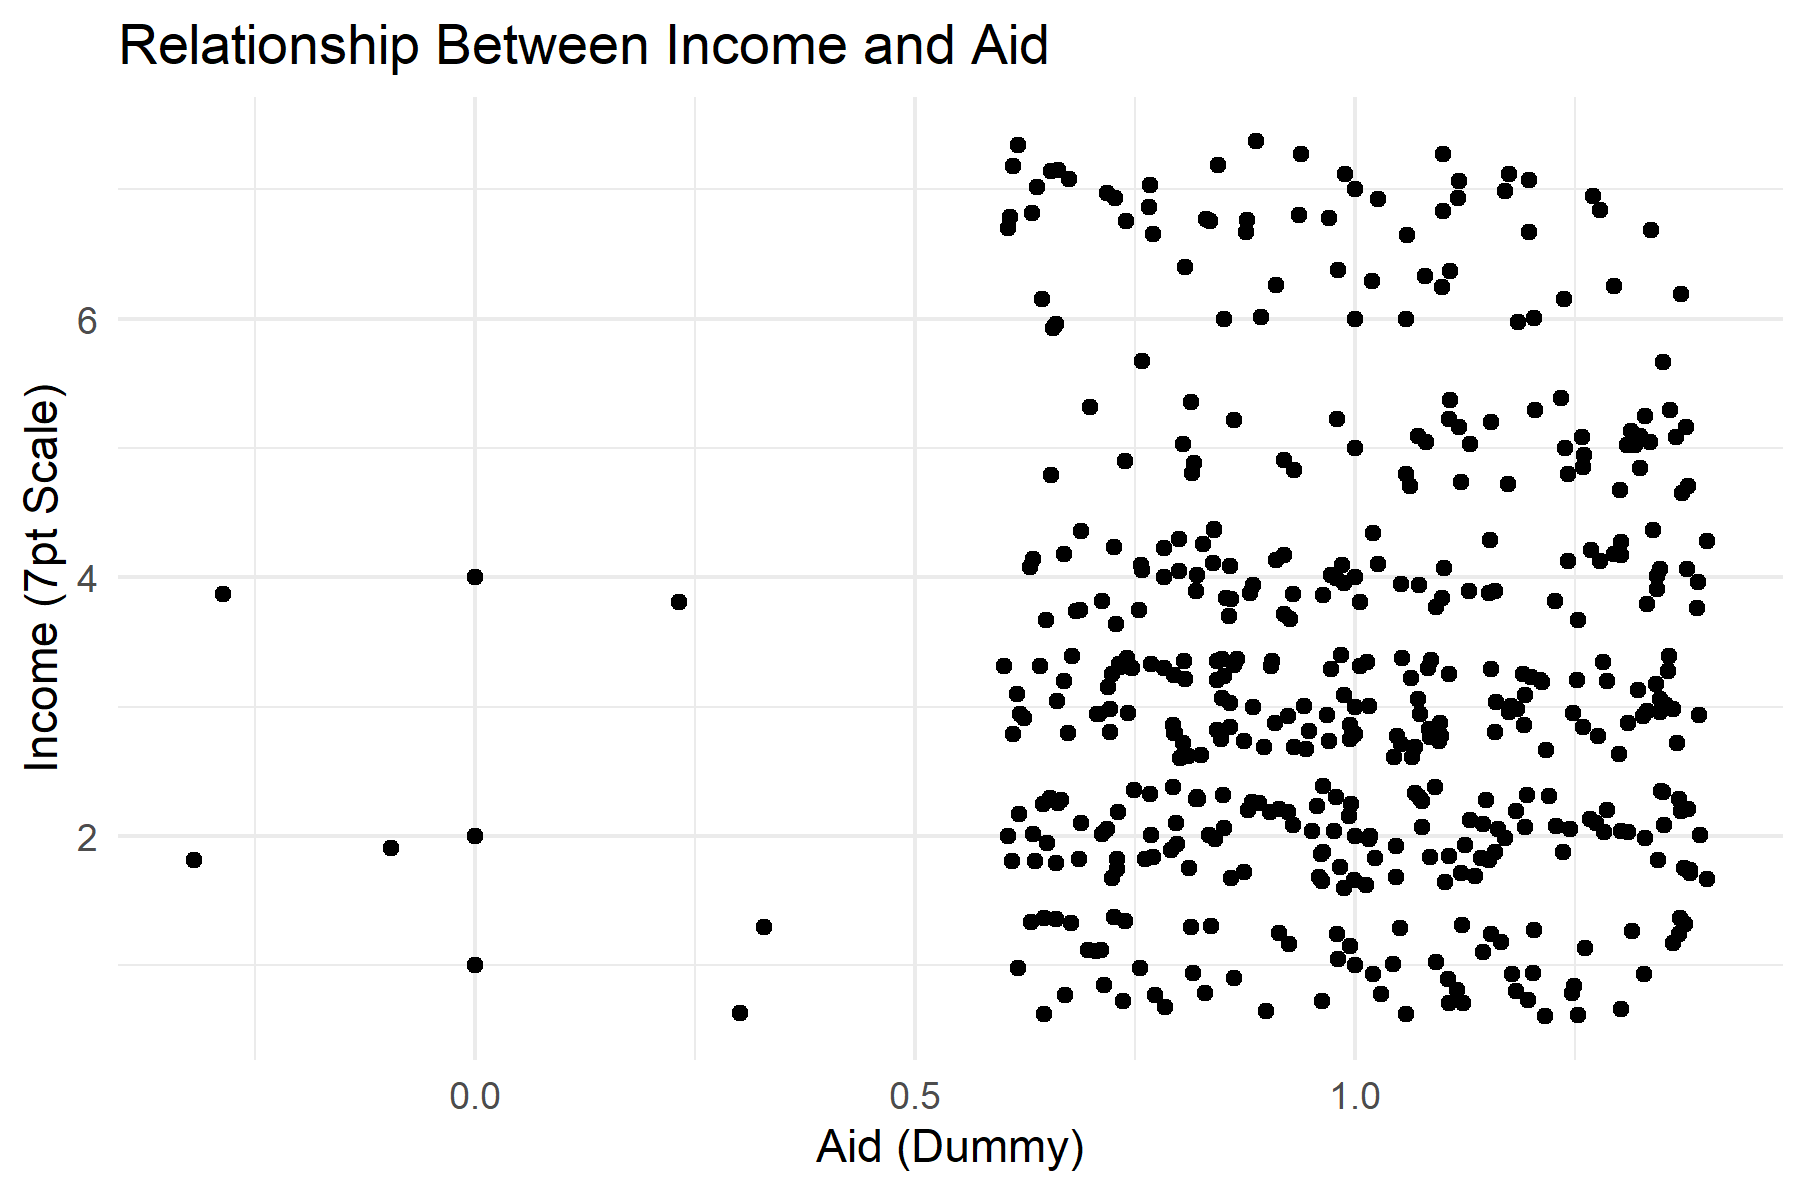
\includegraphics[scale=0.7]{Figs/aid-and-income.png} \centering
	\caption{Relationship Between Receiving Aid and 7pt Income Scale}
	\label{}
\end{figure}

\begin{figure}[H]
	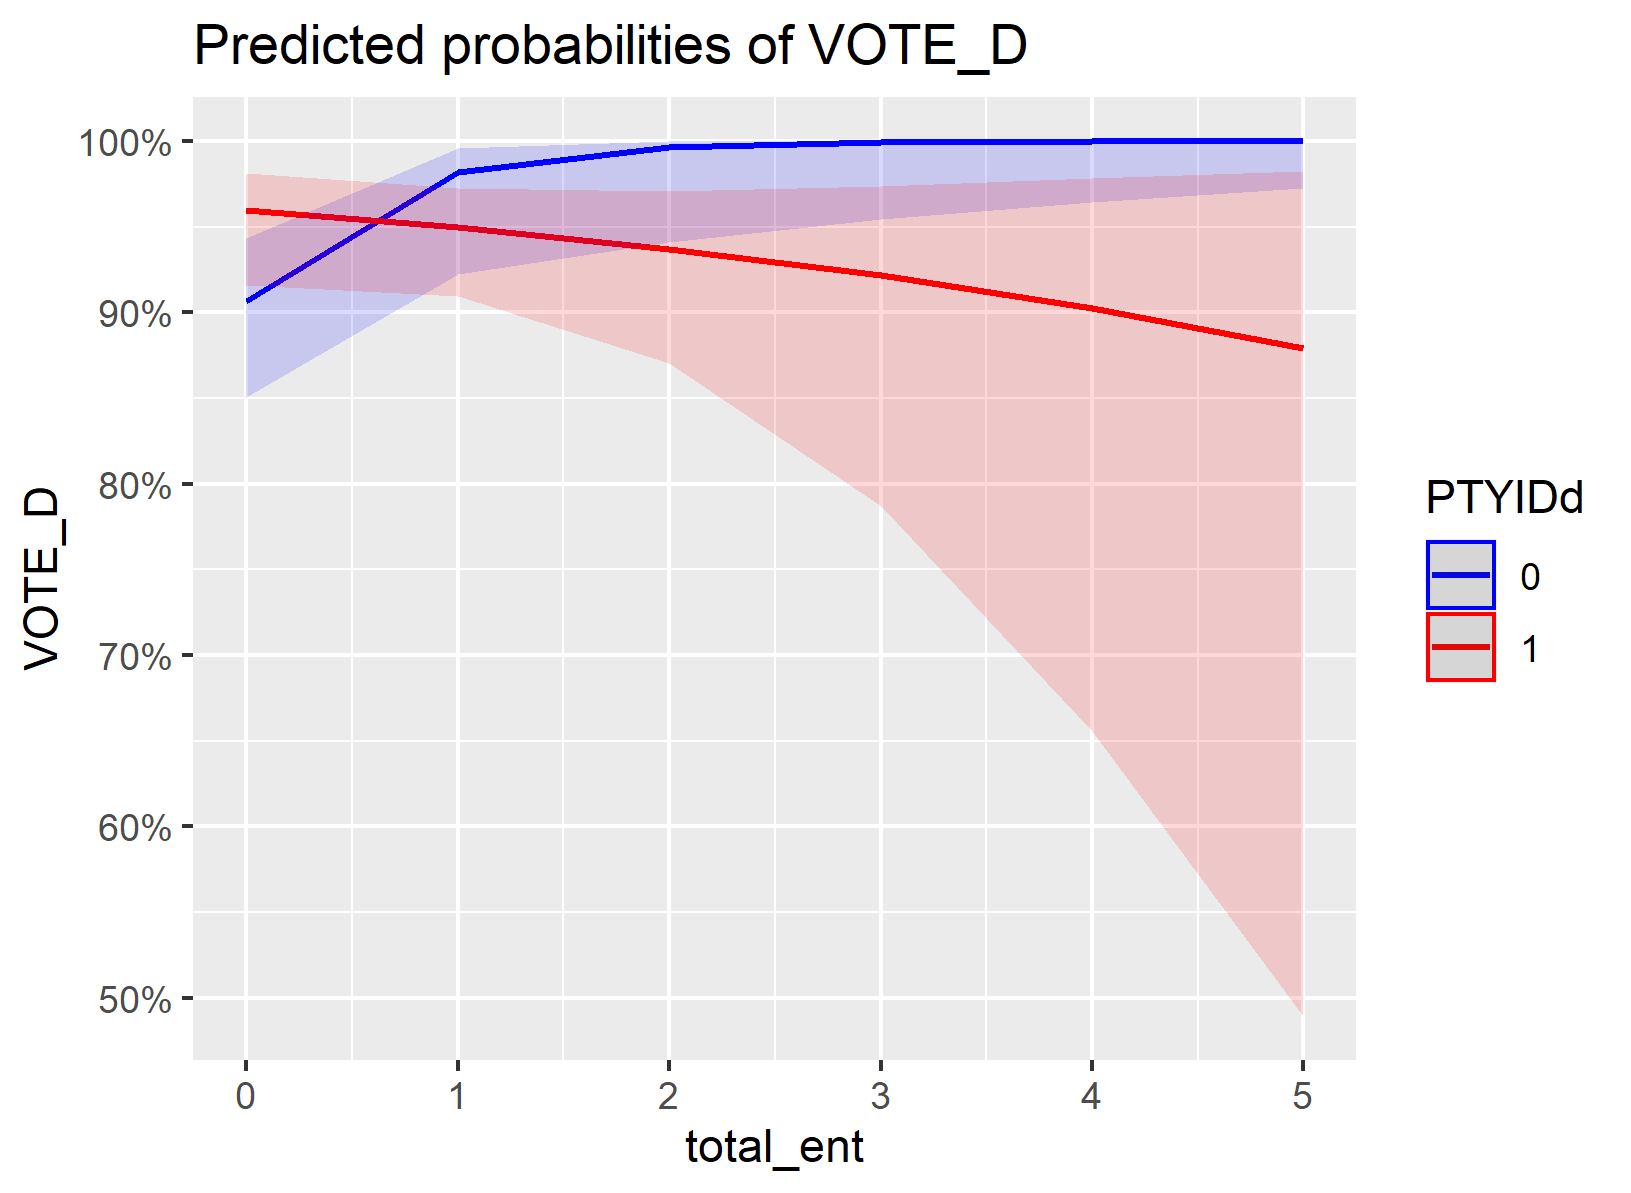
\includegraphics[scale=0.7]{Figs/marginal.png} \centering
	\caption{Marginal Effects of Entitlements on Turnout}
	\label{}
\end{figure}

\begin{table}
\begin{tabular}{l|l}
	\hline
	& max (N = 460)\\
	\hline
	\bf{Vote} & ~\\
	\hline
	~~ Min. & 1\\
	\hline
	~~ Median & 4\\
	\hline
	~~ Mean & 3.65\\
	\hline
	~~ Max. & 4\\
	\hline
	\bf{Republican} & ~\\
	\hline
	~~ Min. & 0\\
	\hline
	~~ Median & 0\\
	\hline
	~~ Mean & 0.47\\
	\hline
	~~ Max. & 1\\
	\hline
	\bf{Self Efficacy} & ~\\
	\hline
	~~ Min. & 0\\
	\hline
	~~ Median & 1\\
	\hline
	~~ Mean & 0.62\\
	\hline
	~~ Max. & 1\\
	\hline
	\bf{Total Aid} & ~\\
	\hline
	~~ Min. & 0\\
	\hline
	~~ Median & 3\\
	\hline
	~~ Mean & 3.75\\
	\hline
	~~ Max. & 13\\
	\hline
	\bf{Total Universal Aid} & ~\\
	\hline
	~~ Min. & 0\\
	\hline
	~~ Median & 0\\
	\hline
	~~ Mean & 0.45\\
	\hline
	~~ Max. & 3\\
	\hline
	\bf{Total Means-Tested Aid} & ~\\
	\hline
	~~ Min. & 0\\
	\hline
	~~ Median & 1\\
	\hline
	~~ Mean & 1.36\\
	\hline
	~~ Min. & 8\\
	\hline
	\bf{Total Entitlements} & ~\\
	\hline
	~~ Min. & 0\\
	\hline
	~~ Median & 0\\
	\hline
	~~ Mean & 0.75\\
	\hline
	~~ Max. & 5\\
	\hline
	\bf{Total Loans} & ~\\
	\hline
	~~ Min. & 0\\
	\hline
	~~ Median & 0\\
	\hline
	~~ Mean & 0.27\\
	\hline
	~~ Max. & 2\\
	\hline
\end{tabular}
\caption{Measures of Central Tendencies for Key Variables}
\label{Appendix C.1}
\end{table}

\begin{figure}[H]
	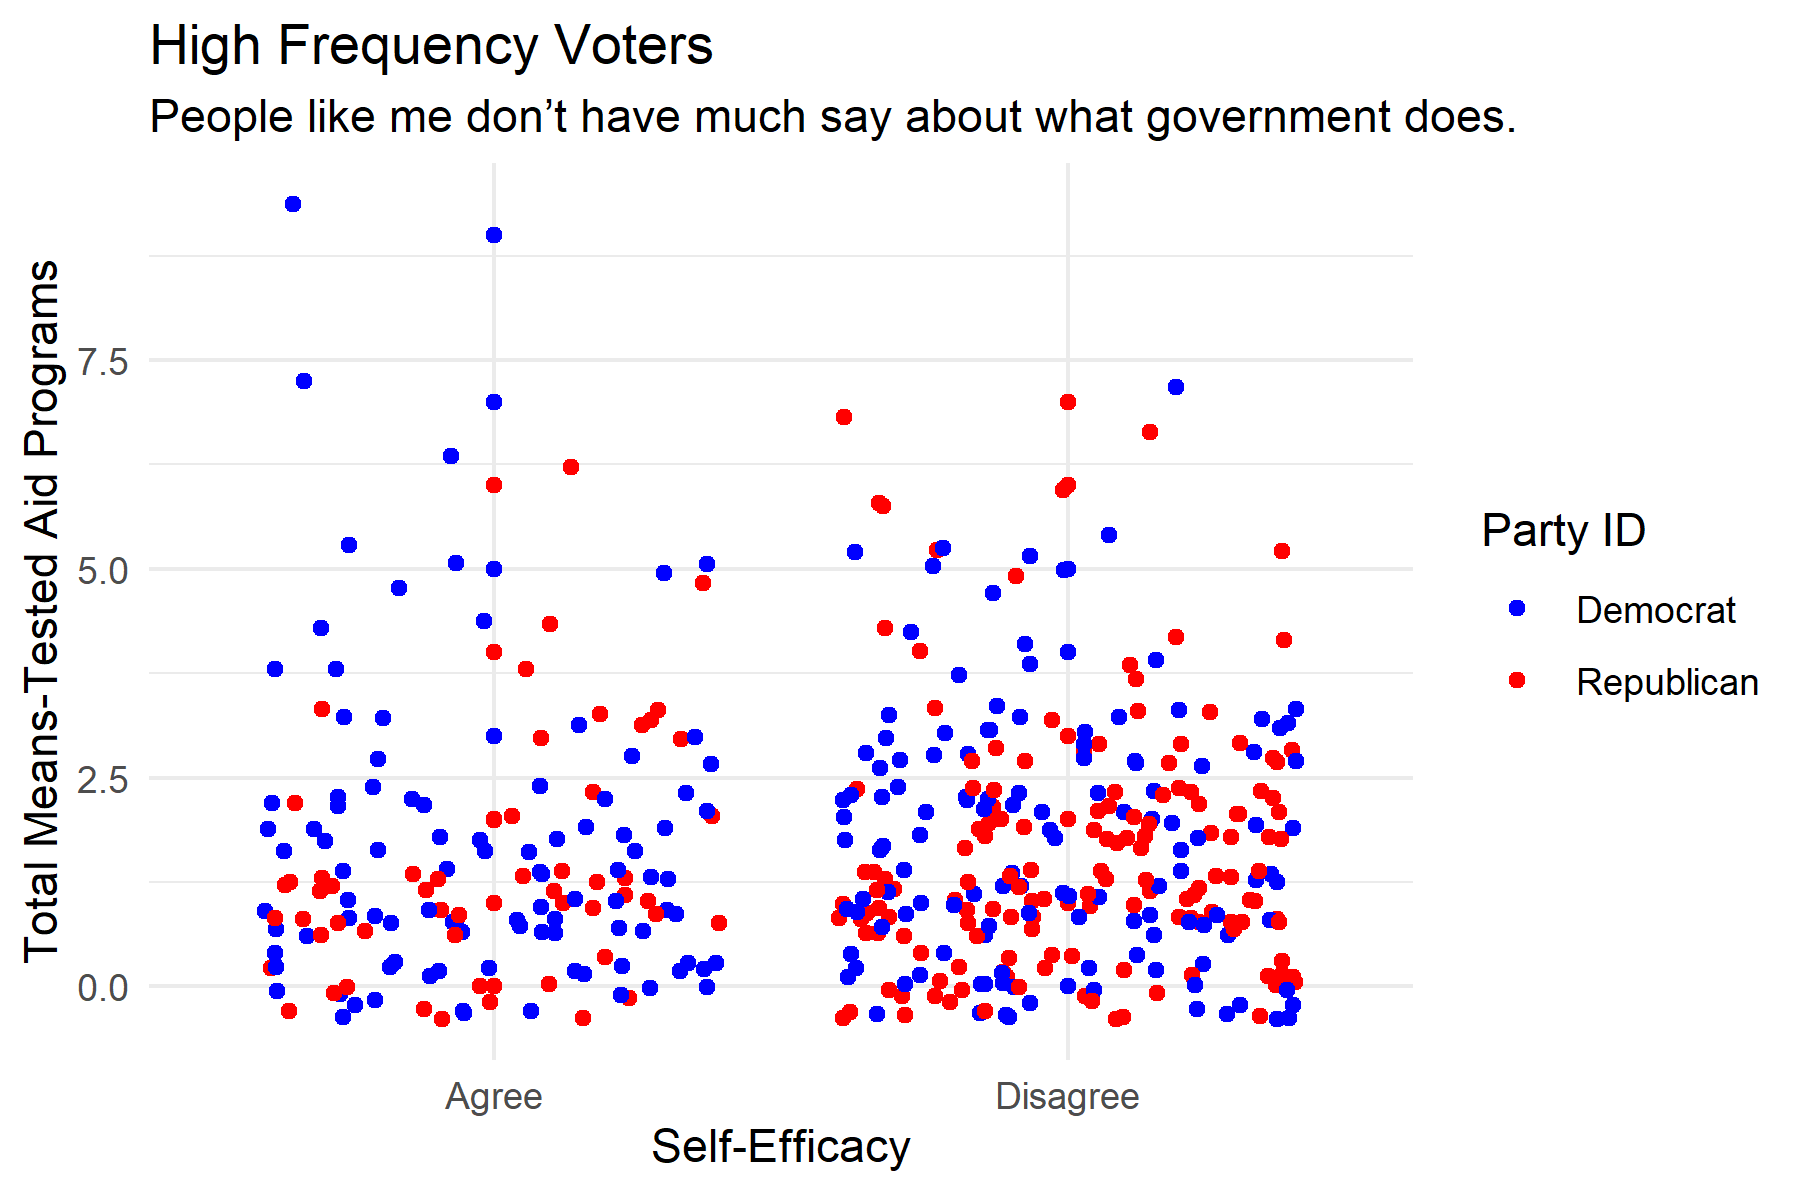
\includegraphics[scale=0.7]{Figs/scatter_means_efficacy_high.png} \centering
	\caption{Self Efficacy Among High-Turnout Voters on Means-Tested Aid}
	\label{}
\end{figure}


\begin{figure}[H]
	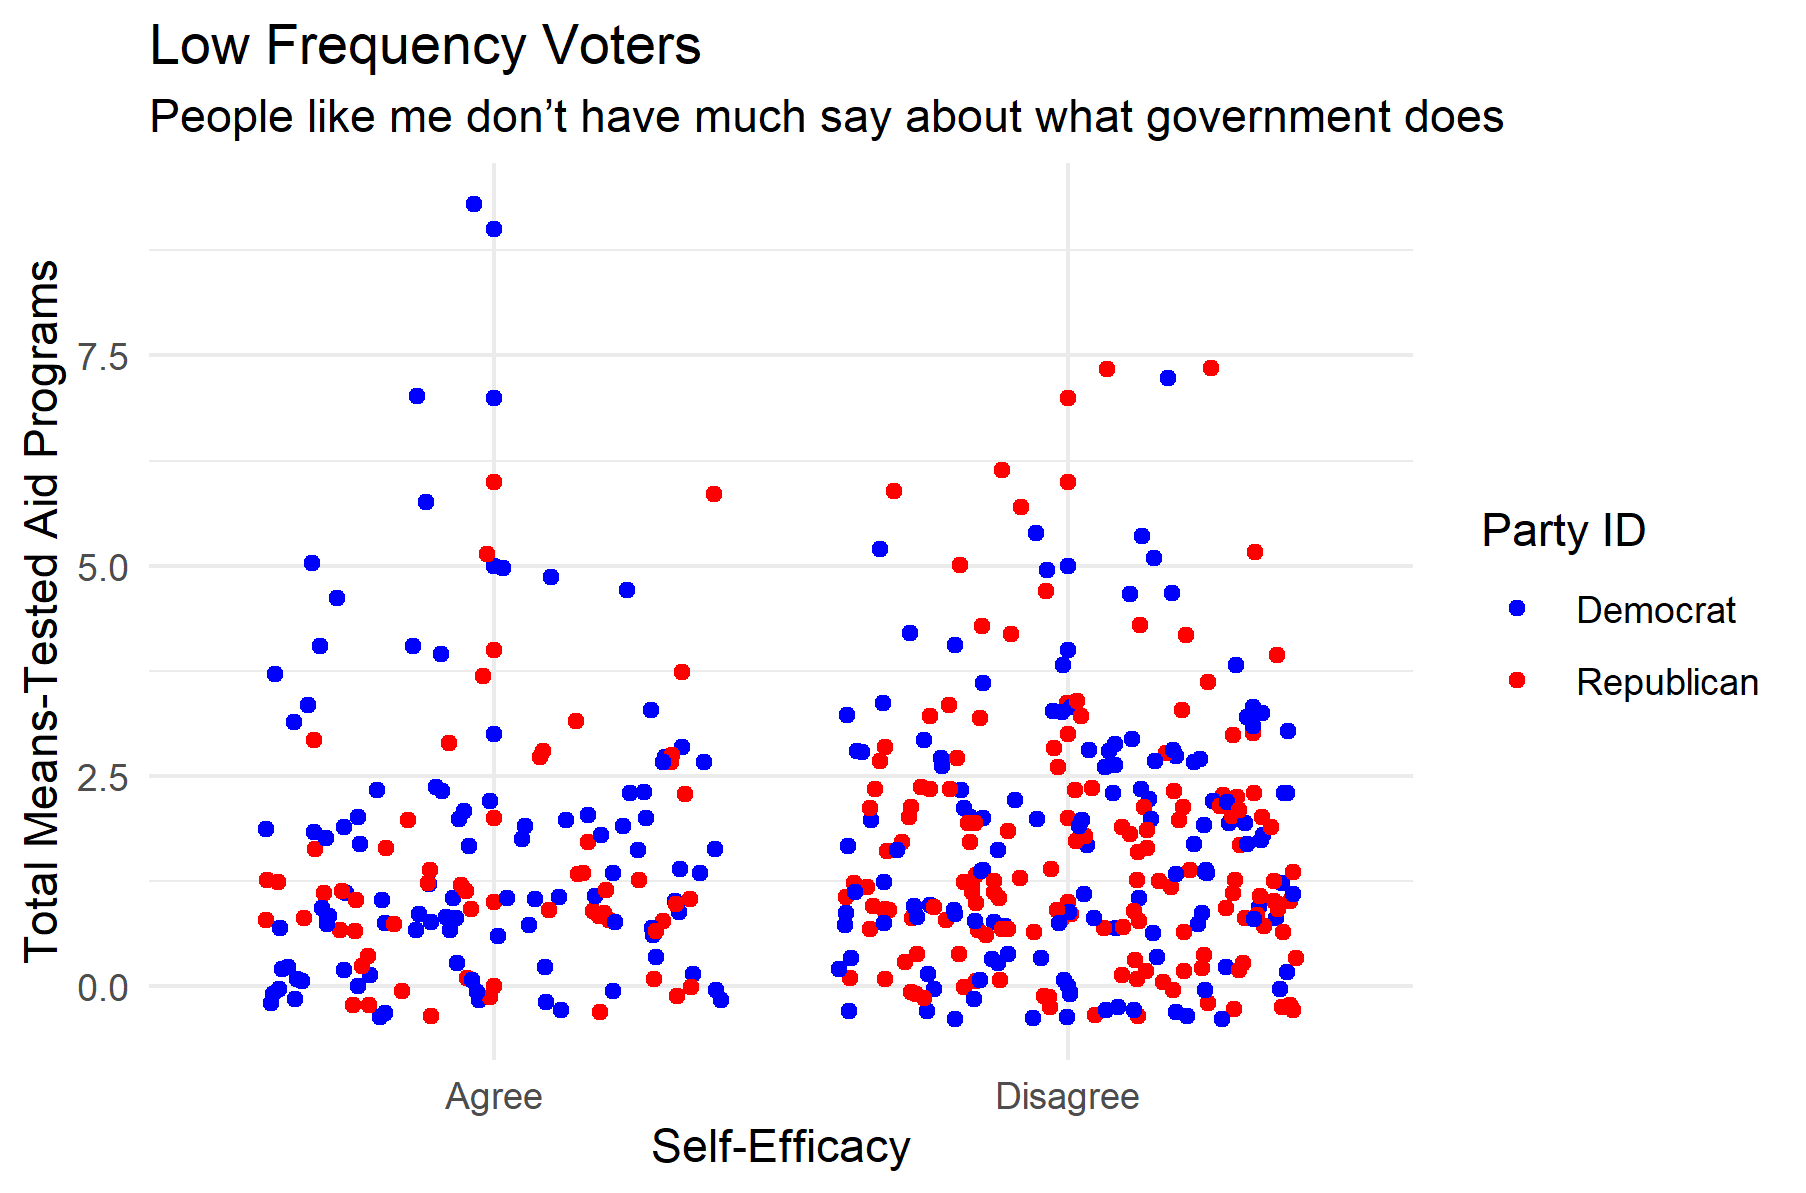
\includegraphics[scale=0.7]{Figs/scatter_means_efficacy_low.png} \centering
	\caption{Self Efficacy Among Low-Turnout Voters on Means-Tested Aid}
	\label{}
\end{figure}

\begin{figure}[H]
	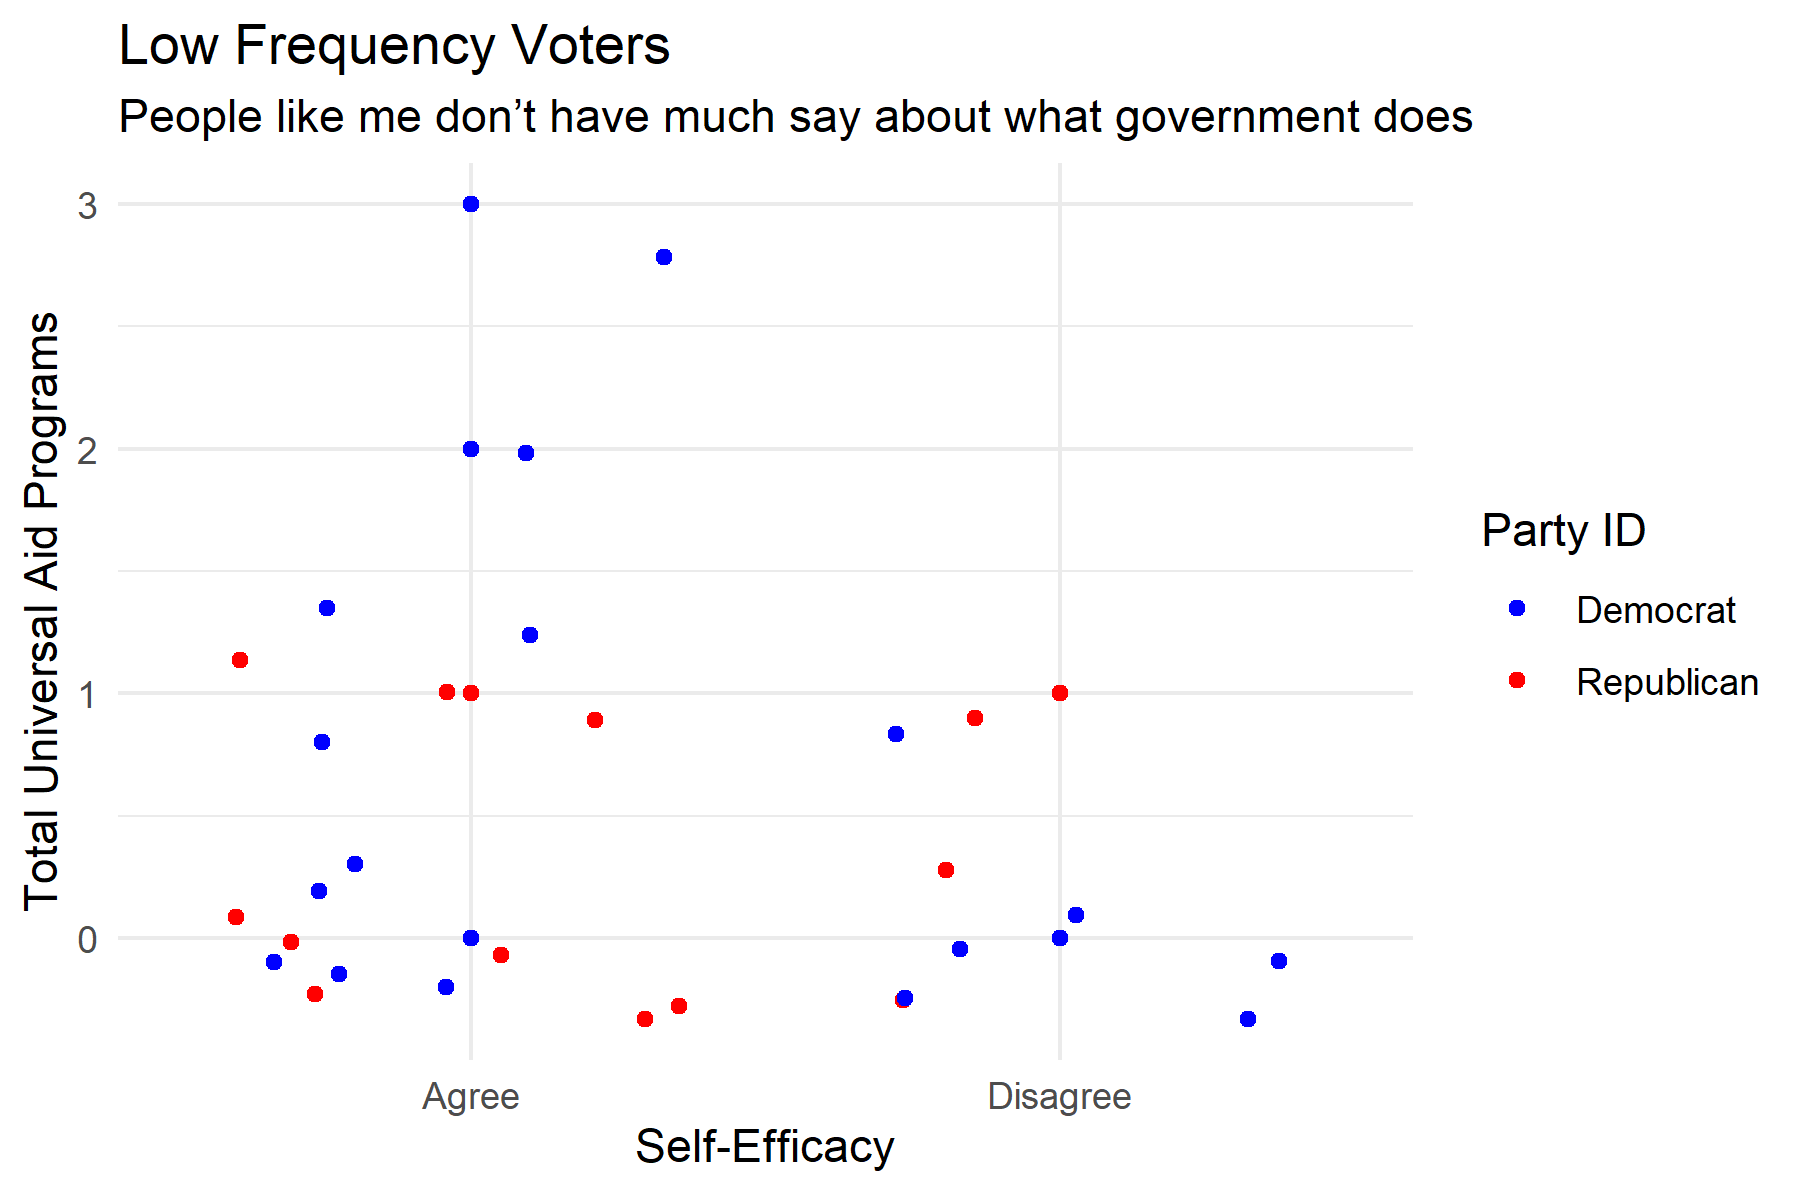
\includegraphics[scale=0.7]{Figs/scatter_uni_efficacy_low.png} \centering
	\caption{Self Efficacy Among Low-Turnout Voters on Universal Aid}
	\label{}
\end{figure}

\begin{figure}[H]
	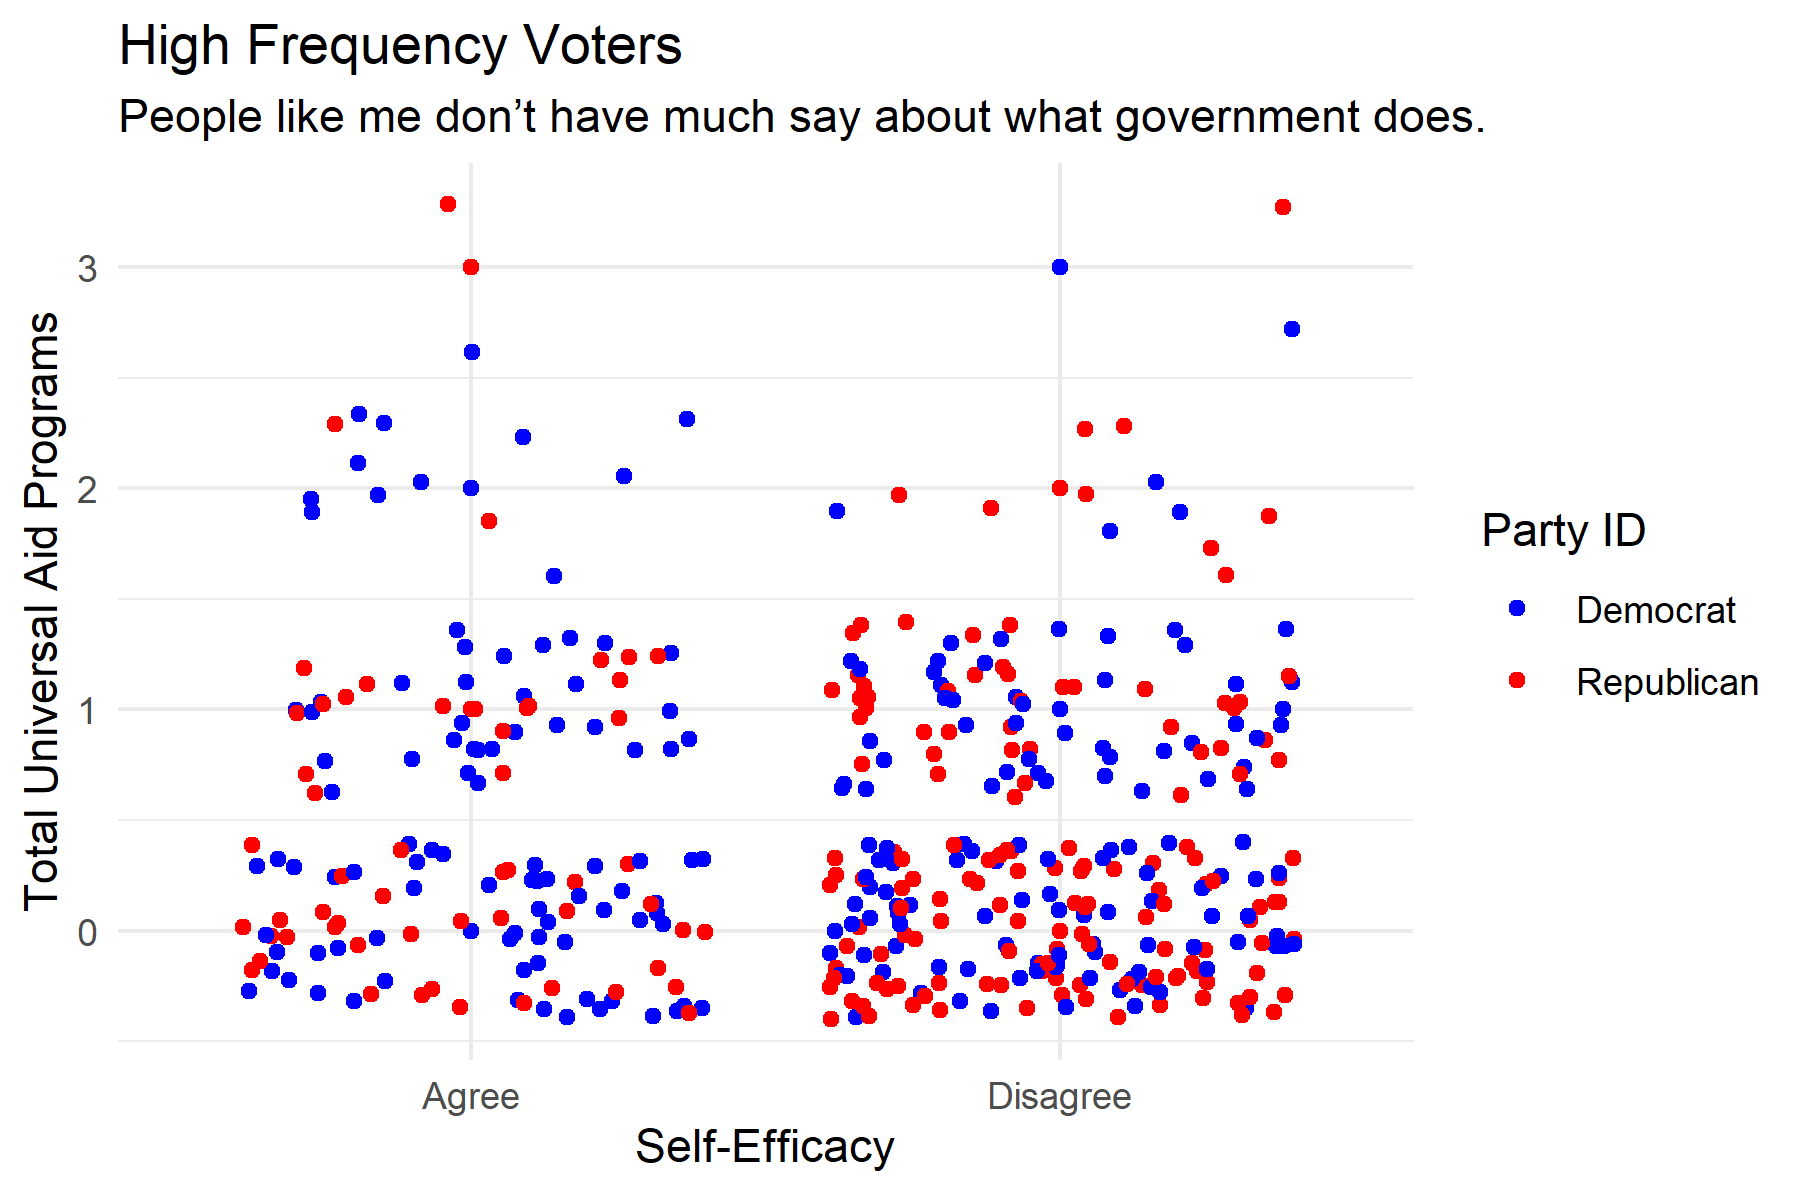
\includegraphics[scale=0.7]{Figs/scatter_uni_efficacy_high.png} \centering
	\caption{Self Efficacy Among High-Turnout Voters on Universal Aid}
	\label{}
\end{figure}

\subsection*{Self Efficacy and Universal Aid}
In Section 2, I reevaluate the self efficacy hypothesis and find that it is not robust to more a more valid measure of aid. In fact, I find that the opposite is true - the relationship between means-testing and self efficacy is statistically insignificant, but then relationship between universal aid and self efficacy is both significant and negative.

To understand this counterintuitive finding, I looked deeper at the data. I plotted the relationship between each of the three universal aid programs and self efficacy. These plots are shown here. While participating in any of the three programs is associated with a lower self efficacy, the relationship is the starkest between SSDI and self efficacy.

\begin{figure}[H]
	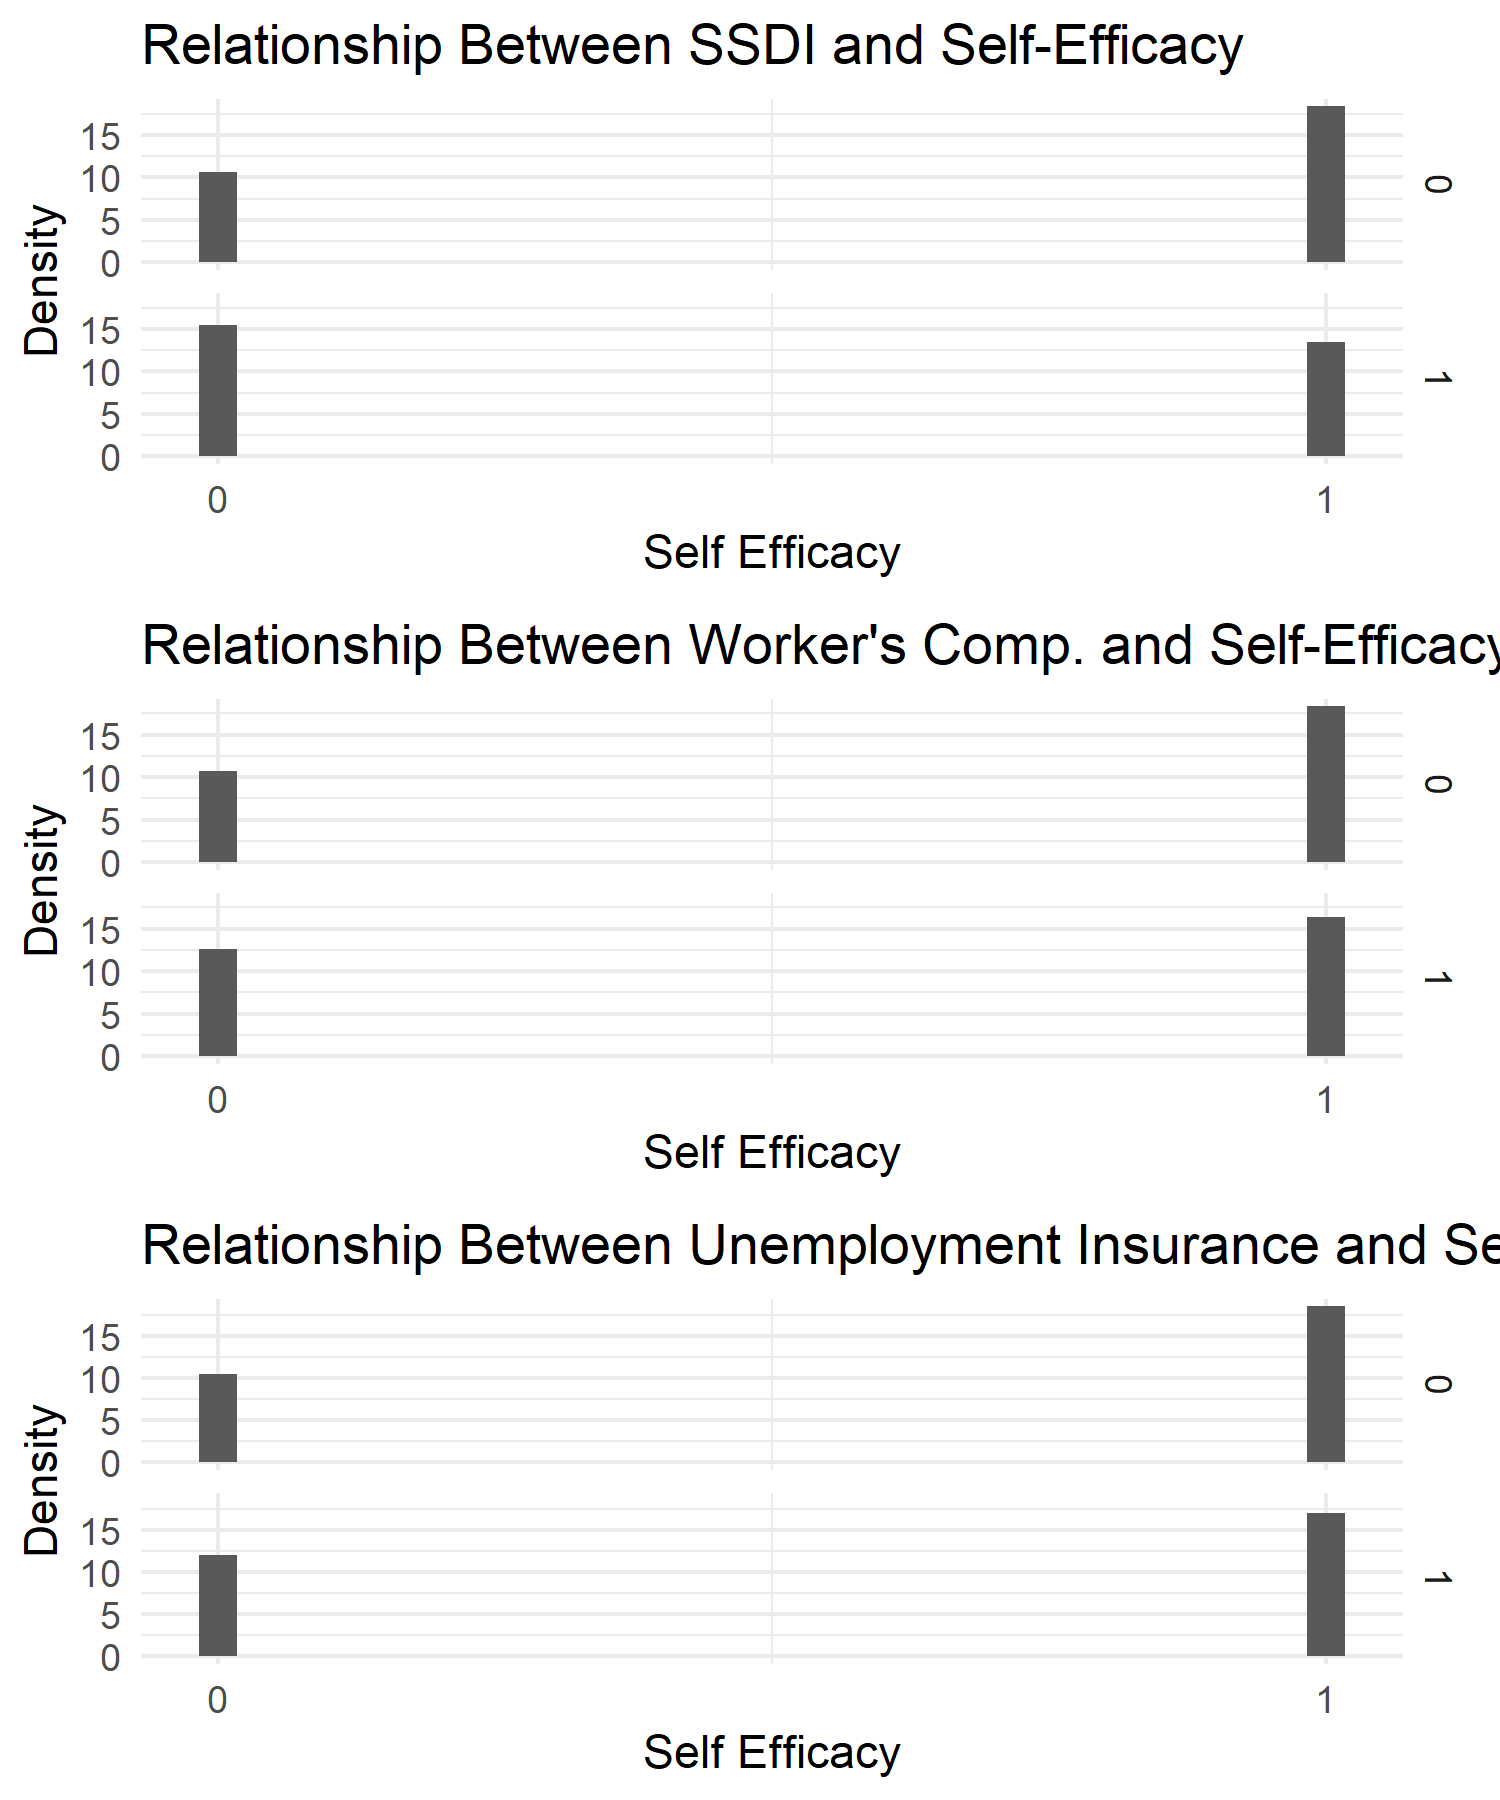
\includegraphics[scale=0.7]{Figs/uni_SE.png} \centering
	\caption{Relationship Between Universal Aid Programs and Self Efficacy}
	\label{}
\end{figure}

\begin{figure}[H]
	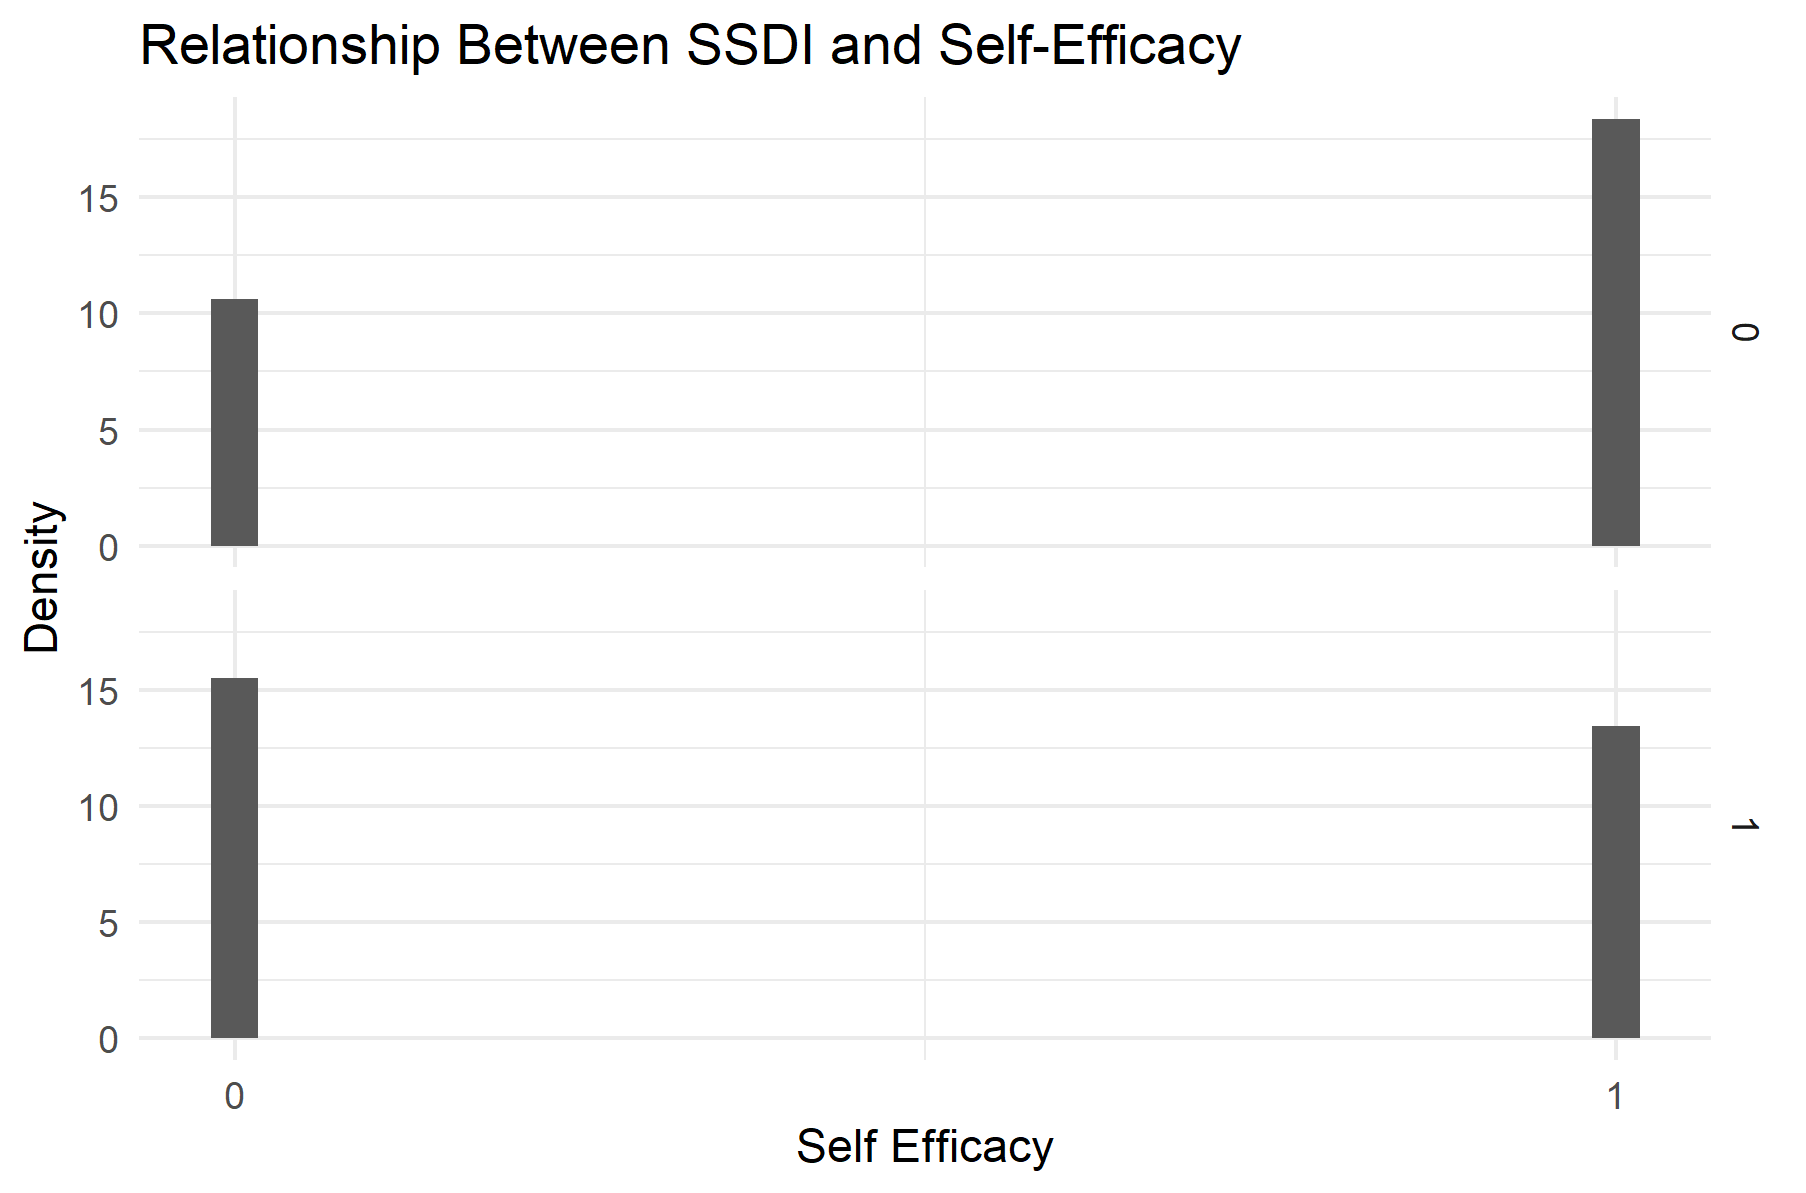
\includegraphics[scale=0.7]{Figs/disability_SE.png} \centering
	\caption{Relationship Between Disability Insurance and Self Efficacy}
	\label{}
\end{figure}

Likely, the traditional dichotomous measure of aid masked this relationship by combining entitlements and universal aid, such that the slight negative effect of certain universal aid programs was empirically ``masked" by the positive relationship between entitlements and self efficacy.

This leads to the question, why are these programs in particular associated with low self efficacy? Previous work assumes that means-testing causes the dip in self efficacy (and therefore the decrease in turnout), but this cannot be the case here because these programs are not means tested. I propose that what we are seeing here is evidence that administrative barriers to aid teach participants that the government does not work for people like them.

I formally develop this theory in Section 3.2 and Appendix A, but discuss the intuition here in light of my cursory analysis. Some aid programs come at a high cost to participants. These costs are upfront and sometimes continuous; they usually come in the form of eligibility requirements. For example, while SSDI is not means tested, potential beneficiaries must provide caseworkers with complete lists of treatment and medication history, employment histories, tax information, and interviews. For particularly complicated cases or for those without support at home in keeping and categorizing the necessary materials, getting aid is incredibly challenging. I argue that these upfront costs associated with certain programs offset or altogether negate the value of aid to participants. If receiving aid mobilizes participants to participate politically, does the cost of aid demobilize voters?

Developing valid and reliable measures of administrative barriers to aid and testing the relationship between aid and these costs should be the focus of future work on this topic.

\section*{Appendix D - Model Proofs}
For simplicity, I assume that Voter V resolves indifference in favor of abstaining.

\textbf{Lemma 1:} In each period $t \epsilon \{1,2\}$, the office-holding executive, $p \epsilon \{I,C\}$, chooses the distributive policy: 
\begin{gather}
x_t=\theta_j (1-p)+ \theta_i (p), 
\end{gather}

where $\theta_j$ is the opposite of the office holder’s type. Incumbent types are therefore not fully separating.

\textbf{Lemma 2:}  After observing the Incumbent’s choice of $y_1 \epsilon {0,1}$ during the first period, the Voter V’s updated belief about the Incumbent’s type is: 
\begin{gather}
p_{(\theta_I)}(p(\theta_i ) + (1 - p)(\theta_j ) | y_1 )=y_1(p)
\end{gather}

Given Lemma 2, V expects to receive $E(y_2 | e=I) = p(\theta_i )+(1-p)(\theta_j)$ units of aid in $t=2$ if I is reelected and $E(y_2 |e=C)=E(\theta_C )=\frac{1}{2}$ units of aid if C wins the election.  V’s expected second period payoff from I’s reelection would be: $EU_V (e=I) = -(1 - x_v ) + [p(y_1 ) + (1 - p)(y_1 )]$ whereas his expected second period payoff from C’s election would be: $EU_V (e=C) = - x_V + \frac{1}{2}$. 

Therefore, conditional on turning out, V votes for I iff: 
\begin{gather}
EU_V (e=I) \geq EU_V (e=C) \Rightarrow
x_V \geq -\frac{3 - 2py_1 - 2y_{-1} - 2py_{-1}}{4}
\end{gather}

When $x_V$ is above the threshold, V prefers that the Incumbent win the election, so V’s total expected payoff from voting would be:
\begin{gather}
EU_V (v=1 | x_V \geq -\frac{3 - 2py_1 - 2y_{-1} - 2py_{-1}}{4} =
- (1 - x_V ) + y_1 - c
\end{gather}

When $x_V$ is below the threshold, V prefers that the Challenger win the election, so V’s total expected payoff from voting would be:
\begin{gather}
EU_V (v=1 | x_V < -\frac{3 - 2py_1 - 2y_{-1} - 2py_{-1}}{4} = 
-x_V + \frac{1}{2} - c
\end{gather}

V’s total combined expected payoff from not voting is:
\begin{gather}
EU_V (v=0) = \frac{EU_V (e=I)}{2} + \frac{EU_V (e=C)}{2} = 
\frac{y_1}{2} - \frac{1}{4}
\end{gather}

Hence, in equilibrium, V turns out to vote iff: $EU_V (v=1) \geq EU_V (v=0) \Rightarrow c \leq \bar{c}$ where:

\begin{equation}
\bar{c} =
\begin{cases}
\frac{-y_1}{2} - x_V + \frac{3}{4} & if x_V < \frac{1}{4} \\
x_V (2y_1 - 1) + \frac{3}{4}     & if \frac{1}{4} \leq x_V < \frac{3}{4}  \\
\frac{y_1}{2} + x_V - \frac{3}{4}     & if x_V \geq \frac{3}{4}  \\
\end{cases}
\end{equation}

\textbf{Lemma 3:}
Given turning out, V’s vote in the election is:
\begin{equation}
s =
\begin{cases}
I, & if x_V \geq -\frac{3 - 2py_1 - 2y_{-1} - 2py_{-1}}{4} \\    
C,     & otherwise  \\
\end{cases}
\end{equation}
where $y_{-1}$ is the aid amount not delivered in the period (i.e. if $1$ unit of aid was delivered, $y_{-1} = 0$.) This demonstrates the consequence of candidate types not fully separating in equilibrium: it is entirely possible that the Voter could oust an Incumbent of type $\theta_I = 1$ and keep an incumbent of type $\theta_I = 0$ due to a bad signal.\footnote{If the Incumbent's actions were not determined probabalistically, but were instead allowed to vary their aid policy strategically, it follows, then, that Incumbents would deliver the minimum amount of aid necessary to satisfy the Voter's threshold for $x_v > \frac{1}{2}$ and the minimum amount of aid necessary to repress turnout for $x_v < \frac{1}{2}$.}


\textbf{Lemma 4:} Let $P_(y_1 )(x_V )$ denote the probability of turnout for a voter with ideal point $x_V$ and who receives $y_1 \epsilon \{0,1\}$ of aid during Period 1. V’s turnout choice in the election is:

\begin{equation}
P_(y_1 )(x_V ) =
\begin{cases}
\frac{-y_1}{2} - x_V + \frac{3}{4} & if x_V < \frac{1}{4}\\    
x_V (2y_1 - 1) + \frac{3}{4}     & if \frac{1}{4} \leq x_V < \frac{3}{4}  \\
\frac{y_1}{2} + x_V - \frac{3}{4}     & if x_V \geq \frac{3}{4}  \\
\end{cases}
\end{equation}

Given this, we can calculate the \emph{change in turnout probability} from receiving one unit of aid in $t_1$. Put differently, the effect of receiving $y_1 = 1$ is:
\begin{equation}
P_1 (x_V ) - P_0 (x_V )=
\begin{cases}
\frac{-1}{2} & if x_V < \frac{1}{4}\\    
2x_V - 1 & if \frac{1}{4} \leq x_V < \frac{3}{4}  \\
\frac{1}{2} & if x_V \geq \frac{3}{4}  \\
\end{cases}
\end{equation}

\end{document}